\documentclass[oneside]{book}
\bibliographystyle{plain}
%\bibliographystyle{apalike}
\setlength{\headheight}{10pt}
\usepackage[ngerman]{babel}
\usepackage{graphicx}
\usepackage{lscape}
\usepackage{caption}
\usepackage{longtable}
\usepackage{setspace}
\usepackage{listings}
\usepackage{ulem}
\usepackage{float}
\usepackage{titleref}
\usepackage{enumitem}
\usepackage[utf8]{inputenc} 
\usepackage{amsmath}


\usepackage{listings}

\lstset{language=JAVA, breaklines=true, basicstyle=\footnotesize \ttfamily, showspaces=false, showtabs=false, tab= , keywordstyle=\bfseries, showstringspaces=false, framexleftmargin=3mm, frame=single, numbers=left, numberstyle=\tiny, stepnumber=1, numbersep=2pt, texcl=false, escapechar=$,captionpos=b}
%-----------------------------------------------------------
% properties
%-----------------------------------------------------------
\author{Raffael Schmid} 
	

%-----------------------------------------------------------
% design
%-----------------------------------------------------------




%-----------------------------------------------------------
% document
%----------------------------------------------------------
\begin{document}
\begin{titlepage}
\begin{center}
\textsc{\Huge \bf Bachelorthesis}\\[0.4cm]
\LARGE \textbf{Konzeption und Entwicklung eines Auswertungstools für die Log Files des JRockit Garbage Collectors}\\[1.0cm]
\large \textbf{von}\\[0.5cm]
\large \textbf{Raffael Schmid}\\[3cm]
\LARGE Aufgabenstellung\\
\vspace{7cm}

\end{center}

\begin{tabular}[ht]{ll}
  Schule: & Hochschule für Technik, Zürich\\
  Betreuer: & Mathias Bachmann\\
  Experte: & Marco Schaad \\
  Zeitraum: & 22. Juni 2011 - 22. Dezember 2011
\end{tabular}
\end{titlepage}

\chapter*{Abstract}
Die vorliegende Bachelorthesis befasst sich mit der Anforderungsanalyse, Konzeption und Implementation einer Software zur Analyse von Garbage Collection Logdateien der JRockit virtual Machine.
\tableofcontents
\chapter*{Einleitung}
Bei der Performanceanalyse einer Software kann es notwendig sein, das  Verhalten der Garbage Collection genauer zu betrachten. Diese Auswertung kann mit der Software JRockit Mission Control im laufenden Betrieb oder danach auf der Basis von resultierenden Logdateien gemacht werden. Im zweiten Fall gibt es allerdings - zumindest für die JRockit Virtual Machine (Release 28) keine Werkzeuge zur Automation dieser Aufgaben. Die vorliegende Bachelorthesis zeigt das Konzept und die Implementation einer Analysesoftware für Garbage Collection Logs der JRockit Virtual Machine. Die Software soll so erweiterbar sein, dass sie auch für andere Garbage Collection Algorithmen erweitert werden kann.

Die Bachelorthesis ist in drei Teile gegliedert: Teil eins definiert die von der Schulleitung abgenommene Aufgabenstellung, Teil zwei befasst sich mit der Umsetzung, von der Anforderungsanalyse bis zur Implementation und im dritten Teil befindet sich der Anhang.
\part{Projektbeschreibung}
\documentclass[11pt]{article}
\setlength{\headheight}{10pt}
\usepackage[german, ngerman]{babel}
\usepackage[utf8]{inputenc} 
\usepackage{fancyhdr}
%-----------------------------------------------------------
% properties
%-----------------------------------------------------------
\author{Raffael Schmid} 


%-----------------------------------------------------------
% design
%-----------------------------------------------------------




%-----------------------------------------------------------
% document
%-----------------------------------------------------------
\begin{document}
\lhead{\textit{leftheader}}
\begin{titlepage}
\begin{center}
\textsc{\Huge \bf Bachelorthesis}\\[0.4cm]
\LARGE \textbf{Konzeption und Entwicklung eines Auswertungstools für die Log Files des JRockit Garbage Collectors}\\[1.0cm]
\large \textbf{von}\\[0.5cm]
\large \textbf{Raffael Schmid}\\[3cm]
\LARGE Protokoll Design Review\\
\vspace{7cm}

\end{center}

\begin{tabular}[ht]{ll}
  Schule: & Hochschule für Technik, Zürich\\
  Betreuer: & Matthias Bachmann\\
  Experte: & Marco Schaad \\
  Zeitraum: & 22. Juni 2011 - 22. Dezember 2011
\end{tabular}
\end{titlepage}

\section{Teilnehmer}
\begin{itemize}
	\item Olaf Stern (Schulleiter)
	\item Matthias Bachmann (Betreuer)
	\item Raffael Schmid (Student)
\end{itemize}
\section{Einleitung}
Mit der Bachelorthesis möchte der Student Raffael Schmid sein Studium an der Hochschule für Technik abschliessen. Als Thema hat er die Konzeption und Implementation eines Auswertungswerkzeugs für Garbage Collection Logs der JRockit Virtual Machine gewählt. 

\section{Ablauf}
\begin{enumerate} 
\item \textbf{Begrüssung} - Die Teilnehmer begrüssen sich und definieren kurz den Ablauf des Kickoffs.
\item \textbf{Präsentation Thema} - Der Student Raffael Schmid stellt Thema, Ausgangslage, Ziele der Arbeit, Aufgabenstellung und erwartete Resultate basierend auf der eingegebenen Aufgabenstellung vor.
\item \textbf{Überprüfung "Checkliste für die Aufgabenstellung einer Bachelorarbeit"} - Anhand der Checkliste wird festgestellt, dass die Aufgabenstellung alle deren Punkte erfüllt.
\item \textbf{Diskussionsrunde} - Die Teilnehmer diskutieren verschiedene Punkt. Siehe dazu \titleref{besonderes}.
\end{enumerate}

\section{Besonderes}\label{besonderes}
\subsection{Schwerpunkt konzeptioneller Teil}
Seitens Schulleitung wurde nochmals erwähnt, dass der Schwerpunkt der Bachelorarbeit auf dem konzeptionellen Teil liegt.
\subsection{Wissenschaftliche Arbeitstechnik}
Bei Problemen respektive Entscheiden während der Umsetzung sollen die verschiedenen Möglichkeiten aufgezeigt werden. Vor- und Nachteile der verschiedenen Lösungsansätze sollen dokumentiert und die resultierenden Entscheidungen nachvollziehbar sein.
\subsection{Zusammenarbeit mit dem Betreuer}
Die Kommunikation von Betreuer und Student findet massgeblich an folgenden Terminen statt:
\begin{enumerate}
	\item Mitte bis Ende August: Informelles Meeting Überprüfung Requirements Engineering
	\item Mitte bis Ende September: Design Review (offizieller Termin)
	\item Mitte Dezember: Abgabe, Präsentation (offizieller Termin)
\end{enumerate}
\subsection{Abgabetermin}
Im neuen Reglement ist der Abgabetermin der Bachelorthesis mit 6 Monaten nach Freigabe der Aufgabenstellung definiert. Da es vorher in den Reglementen kleine inkonsistenten gab (als Starttermin wurde auch Kickoff-Datum erwähnt), wurde der Start-Termin auf den 22. Juni 2011 (Tag des Kickoffs) festgelegt.


\end{document}

\chapter{Analyse der Aufgabenstellung}\label{analyse_aufgabenstellung}
Das Ziel dieser Arbeit ist die Konzeption und Implementation einer Software für die Analyse von Garbage Collection Logdateien der JRockit Virtual Machine. Die grosse Datenmenge soll schnell eingelesen und übersichtlich, informativ dargestellt werden. 

Um die Anforderungen an diese Software zu ermitteln, werden im Bereich der Performanceanalyse, der Garbage Collection und über die JRockit Virtual Machine die nötigen Grundlagen erarbeitet. Anschliessend wird die Anforderungsanalyse durchgeführt. Aufbauend auf dieser kann die Stärken-/Schwächen-Analyse und die Evaluation der bestehenden Rich Client Framworks und Bibliotheken zur Generierung von Diagrammen gemacht werden. Es folgt die Konzeption, Implementation und das Review (Synthese) der Software. Weitere Einzelheiten zu den Teilaufgaben befinden sich in im weiteren Verlauf dieses Abschnittes.

\section{Erarbeitung der Grundlagen}
Die Erarbeitung der Grundlagen dient als Basis in zwei Bereichen:
\begin{itemize}
	\item \textbf{Anforderungsanalyse:} Aus Sicht des Analysten respektive dem Benutzer dieser Software ist es wichtig, dass er die richtigen Daten der Garbage Collection, die richtige Sicht auf diese Daten hat und geeignet filtern kann. Voraussetzung für diese Anforderungen sind die Kenntnisse der verschiedenen Garbage Collection Algorithmen, insbesondere der JRockit VM. 
	\item \textbf{Konzept: } Die Konzeption des Domänen-Modells und des Parseprozesses der Logdateien bedingt eine gute Kenntnis des Aufbaus der VM im Bereich des Speichermanagements.
\end{itemize}

\section{Anforderungsanalyse Software-Prototyp}
Die Anforderungen werden zusammen mit einem Performance-Analysten ermittelt und nach \cite[4.3.2 Angepasste Standardinhalte]{pohl2010basiswissen} dokumentiert. Laut dem IEEE\footnote{Institute of Electrical and Electronic Engineers} und \cite[4.5 Qualitätskriterien für das Anforderungsdokument]{pohl2010basiswissen} müssen Anforderungen folgende Kriterien erfüllen:
\begin{itemize}
	\item Eindeutigkeit und Konsistenz
	\item Klare Struktur
	\item Modifizierbarkeit und Erweiterbarkeit
	\item Vollständigkeit
	\item Verfolgbarkeit
\end{itemize}

\section{Stärken-Schwächen-Analyse Rich Client Frameworks}
Die Applikation wird als Rich Client implementiert. Als Basis kommen die Frameworks Netbeans und Eclipse in Frage. Die Stärken-Schwächen-Analyse soll den Entscheid bei der Evaluation der verwendeten Komponenten herleiten. Die Grundlage für diese Aufgabe ist die Anforderungsanalyse.

\section{Evaluation Frameworks}
Basierend auf der Stärken-Schwächen-Analyse wird ein Entscheid für das jeweilige Framework (Eclipse RCP oder Netbeans RCP)  ausgewählt. Nebst der Auswahl der Rich Client Plattform muss auch eine Bibliothek zur Generierung von Diagrammen evaluiert werden.

\section{Konzeption und Implementation}
Basierend auf den Anforderungen wird das Konzept erstellt und anschliessend die Software im Sinne eines Proof of Concept implementiert. 

\section{Bewertung}
Die Bewertung der Software wird auf Basis der Anforderungen gemacht.



	
\part{Grundlagen}
\chapter{Vorgehen Performanceanalyse}
\section{Motivation}

Die Performance respektive Leistungsfähigkeit einer Applikation stellt einer der bedeutendsten Qualitätsanforderungen dar. Sie kann nich nur zu verärgerten Benutzern, sondern auch zu einer Verlangsamung der Business-Prozesse führen. Die Motivation für eine Performanceanalyse entsteht, wenn die in Service Level Agreement oder Anforderungsanalyse spezifizierten \textbf{Qualitätsanforderungen nicht erfüllt} sind. Optimal wäre, wenn diese Anforderung während des Entwicklungsprozesses kontinuierlich geprüft würde.

\section{Ablauf}
Die Performanceanalyse ist ein iterativer Prozess und sollte so lange dauern, bis die Anforderungen erfüllt und der Kunde zufrieden ist. Sie besteht aus folgenden vier Schritten\cite{hummelBeer201109}:
\begin{enumerate}
	\item Identifikation der neuralgischen Punkte des Systems
	\item \textbf{Suche nach dem Dominating Consumer\footnote{Kirk Pepperdine bezeichnet die Aktivität, welche dominiert wie die CPU gebraucht wird, als Dominating Consumer . }}
	\item \textbf{Sammeln von Detaildaten}
	\item Lösen des Problems
\end{enumerate}


Damit die Analyse der Garbage Collection zum richtigen Zeitpunkt gemacht wird, sind insbesondere die Punkte zwei und drei wichtig. Sie werden in den folgenden beiden Abschnitten genauer definiert.
\section{Suche nach dem Dominating Consumer}\label{dominating_consumer}
Die Suche nach dem Dominating Consumer kann nach folgendem Schema durchgeführt werden:
\begin{figure}[H]
  	\centering
    	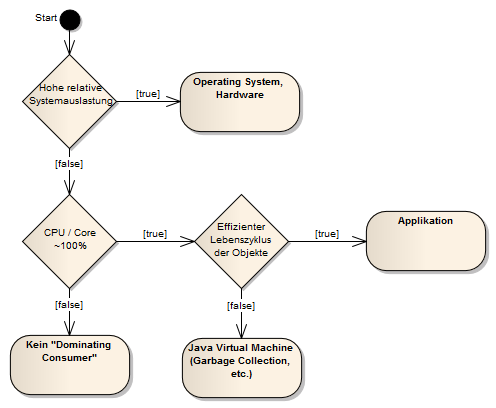
\includegraphics[width=13.1cm]{images/dominating_consumer}
        	\caption{Suche nach dem Dominating Consumer}
\end{figure}

\subsection{Hohe relative Systemlast}\label{hohe_systemauslastung}
Die erste Frage, die sich bei der Suche nach dem Dominating Consumer stellt, ist, ob die hohe CPU-Auslastung\footnote{CPU kann auch einer oder ein paar Cores bedeuten.} durch die Applikation oder das System verursacht wird. Je nach Betriebssystemen gibt es dafür unterschiedliche Werkzeuge:
\begin{itemize}
	\item \textbf{Windows:} Task Manager / Lasche Performance (Leistung). Für die Anzeige der Systemzeit muss die Anzeige der Kernelzeit eingeblendet werden: View / Show Kernel Times
	\item \textbf{Linux / Unix: } vmstat zeigt die Ausnutzung der CPU: vmstat 5
\end{itemize}

Hohe Systemauslastung kann unterschiedliche Gründe haben: 
\begin{itemize}
\item \textbf{Exzessives Context-Switching\footnote{Kontextwechsel}:} Mehrere Prozesse können sich die gleiche CPU (CPU-Kern) nur deshalb teilen, weil beim Wechsel von Prozess A auf B ein Context-Switch gemacht wird, so dass Thread B am selben Ort weiterarbeitet wo er beim letzten Mal war. Gründe für exzessives Context-Switching können beispielsweise nicht adäquat gewählte Locks sein. Wenn ein Thread aufgrund der Synchronisation angehalten werden muss.\footnote{Symptomatisch zeigt dann vmstat, das System ist nicht im Leerlauf, aber die Kernelzeiten (cpu/sy) dominieren die Zeit des Benutzers (cpu/us).}
\item \textbf{Hohe I/O Festplatte} 
\item \textbf{Hohe I/O Netzwerk} 
\end{itemize}


\subsection{Hohe CPU- respektive Core-Last}
Sofern die im Abschnitt \ref{hohe_systemauslastung} beschriebenen Punkte nicht zutreffen, stellt sich die Frage, ob die Auslastung der CPU überhaupt gross ist. Ist das nicht der Fall, gibt es womöglich gar keinen Dominating Consumer - es muss dann herausgefunden werden, was die Threads weg von der CPU haltet. Es gibt dafür laut \cite{pepperdine201102} unterschiedliche Gründe:
\begin{itemize}
\item \textbf{Dead Locks: } Threads schliessen sich gegenseitig aus. 
\item \textbf{Applikation skaliert nicht: } Applikation hat schlechte multi-core Eigenschaften.
\item \textbf{Langsame Disks / Netzwerke}
\item \textbf{Zu kleine Connection- und Thread-Pools}
\item \textbf{Aurufe auf langsame externe Systeme}
\end{itemize}


\subsection{Effizienter Objekt-Lebenszyklus}
Sofern die relative Systemlast klein und die CPU-Auslastung gross ist, muss der Lebenszyklus der Objekte angeschaut werden. Dies kann auf unterschiedliche Arten getan werden:
\begin{itemize}
\item \textbf{Memory Analyse: }Es wird angeschaut, wie alt die Objekte in den verschiedenen Bereiche (Young Collection, Old Collection) sind. Wieviele Garbage Collection Zyklen sie überlebt haben.
\item \textbf{Garbage Collection: }Wann und wie oft werden Garbage Collections durchgeführt, wie lange haben sie gedauert, wieviel Speicher haben sie befreit.
\end{itemize}

\section{Garbage Collection Tuning}
Mit der Analyse des Dominating Consumers entscheidet sich auch, in welchem Bereich anschliessend weitere Detaildaten gesammelt werden. Auch beim Garbage Collection Tuning gilt grundsätzlich: "never change a running system". Man ändert also nur etwas, wenn es Probleme bei der Garbage Collection respektive die Anforderungen daran nicht erfüllt sind. Mit dem Tuning will man in der Regel drei unterschiedliche Ziele erreichen\cite{langerkreftJavaCore}: 
\begin{itemize}
\item Verbesserung des Durchsatzes (siehe Abschnitt \ref{gc_tuning_durchsatz})
\item Geringere Pausenzeiten (siehe Abschnitt \ref{gc_tuning_pausenzeiten})
\item Geringerer Speicherverbrauch (siehe Abschnitt \ref{gc_tuning_speicherverbrauch})
\end{itemize}

Diese drei Ziele bilden eine Dreiecksbeziehung, zum Beispiel führt eine aggressive Optimierung des Durchsatzes in der Regel zu längeren Stop-the-World\footnote{Zeiten in welchen die Prozessoren der Anwendung keine Rechenzeiten zur Verfügung stellen.} Pausen. Tuning bedeutet nun, zwei der Ziele konstant halten, während das dritte durch Anpassung der Konfiguration verbessert wird. Sofern die Optimierung nicht ausreicht, müssen einer oder beide anderen Parameter aufgegeben werden, um das Ziel zu erreichen.


\subsection{Durchsatz\label{gc_tuning_durchsatz}}
Die relative Zeit der CPU welcher der Anwendung zur Verfügung steht nennt man Durchsatz (englisch \textit{Throughput}). Es handelt sich also um einen Prozentsatz im Vergleich mit der gesamten CPU-Zeit. Grundsätzlich ist wird der Durchsatz folgendermassen ausgerechnet:

 \begin{align*}
         Durchsatz &= 100 * (1-Relative\;Zeit\;in\;Garbage\;Collection)\\
         Durchsatz &= 100 * (1-\frac{Zeit\;in\;Garbage\;Collection}{Gesamtdauer\;der\;Messung})
 \end{align*}
Im Prinzip ist diese Formel ziemlich ungenau und berücksichtigt nur die Garbage Collection Zeiten während einer Stop-the-World Pause. Insofern ist sie nur für eine Single-Core CPU genau. Bei einer Multi-Core-Maschine müsste der Througput für jeden einzelnen Core ausgewertet und damit der Gesamt-Throughput berechnet werden.\newline

Durchsatz-Tuning spielt in der Praxis oft nur eine untergeordnete Rolle\cite{langerkreftJavaCore}. Eine wirkliche Steigerung des Durchsatzes kann man nur mit einer aggressiven Optimierung erzielen, sie führt zu verlängerten Pausenzeiten, was nur bei Batch-Applikationen toleriert werden kann. Gleichzeitig ist der Austausch oder das Zuschalten von weiteren CPUs sehr rasch der kostengünstigere Weg.

\subsection{Pausenzeiten\label{gc_tuning_pausenzeiten}}
In der Regel geht es beim Garbage Collection Tuning um das Tuning der Pausenzeiten, dies weil man die Symptome wie Stottern und einer ungleich reaktionsfreudigen Anwendung beseitigen möchte. 

In der Regel startet man mit der Analyse einzelner Garbage Collections. Die Gründe für die Initiierung einer Garbage Collection können sehr unterschiedlich sein und müssen entsprechend behandelt werden:
\begin{itemize}
\item \textbf{Erreichen eines Schwellenwerts des Young- oder Old-Spaces: } Anpassung der Grösse des Young- / Old-Spaces, Vergrösserung des Heaps, etc.
\item \textbf{Heap hat maximale Grösse erreicht:} Anpassung der Heap-Grösse, Beseitigung von Memory Leaks, etc.
\item \textbf{Allokation von Objekten ist nicht möglich:} Vergrösserung des Young-Space, Beseitung der Fragmentierung, etc. 
\item \textbf{Von der Applikation innitiert (System.gc()):} Von der Applikation ausgelöste Garbage Collections können mittels einem Flag ignoriert werden.
\end{itemize}



\subsection{Speicherverbrauch\label{gc_tuning_speicherverbrauch}}
Dieses Tuningziel verliert insofern an relevanz, weil 64-Bit-JVMs bei grossen Applikationen schon sehr verbreitet sind. Mit den 32-Bit Adressen kam man im Bereich des Arbeitsspeichers schon eher an die Grenze (ein Teil des adressierbaren Bereichs von 4GB bei 32-Bit-Adressen wird auch noch Für das Betriebssystem verwendet). Eine Optimierung im Bereich des Speicherverbrauchs hat in der Regel nichts mit Garbage Collection Tuning zu tun, sondern ist eine Analyse der Objektpopulation im Bereich der Applikation.


\chapter{Grundlagen Garbage Collection}
Schon seit den ersten Programmiersprachen ist das Aufräumen von verwendeten Ressourcen / Speicher ein wichtiges Thema. Im Unterschied zu den ersten Sprachen, bei denen das Memory Management in der Verantwortung des Entwicklers war (explizit), findet allerdings das Recycling von Memory bei Sprachen der dritter Generation automatisch statt und macht Operatoren wie ``free'' unwichtig. Bei Formen dieser automatischen Speicherverwaltung spricht man von Garbage Collection\footnote{vom englischen Wort ``garbage collector'' für Müll-, Abfallsammler}. In den meisten neueren Laufzeitumgebungen spricht man zusätzlich von adaptivem Memory Management was bedeutet, dass Feedback der Laufzeitumgebung zur Anpassung der Garbage Collection Strategie verwendet wird.
Probleme die nur beim expliziten Memory Management auftreten sind  Dangling References/Pointers\footnote{Man spricht von Dangling Pointers oder Dangling References, wenn ein Pointer auf ein Objekt im Memory freigegeben wurde, obwohl es noch gebraucht wird.} und Space Leaks\footnote{Man spricht von Space Leaks, wenn Memory alloziert und nicht mehr freigegeben wurde, obwohl es nicht mehr gebraucht wird.\cite{sunMemoryManagementWP}}. Trotzdem sind Memory Leaks auch bei automatischer Speicherverwaltung noch möglich, nämlich dann wenn Memory noch referenziert wird, auch wenn es schon nicht mehr gebraucht wird.
Der folgende Abschnitt beschreibt die Grundlagen der Java Garbage Collection und geht im zweiten Teil auf die spezifischen Eigenheiten der JRockit Virtual Machine ein.

\section{Funktionsweise}
Alle Techniken der Garbage Collection zielen darauf ab, die ``lebenden'' von den ``toten'' Objekten im Speicher zu unterscheiden. Sprich, es müssen die Objekte gefunden werden, welche innerhalb der Software oder des Systems nicht mehr referenziert werden. Die aktuellen Strategien lassen sich laut\cite[S. 77]{lagergren2010oracle} in zwei unterschiedliche Familien aufteilen: ``Reference Counting'' und ``Tracing techniques''.

\subsection{Reference counting\cite[S. 77]{lagergren2010oracle}}
Beim Reference counting behält die Laufzeitumgebung jederzeit den Überblick, wie viele Referenzen auf jedes Objekt zeigen. Sobald die Anzahl dieser Referenzen auf 0 gesunken ist, wird das Objekt für die Garbage Collection freigegeben. Trotzdem der Algorithmus relativ effizient ist, wird er aufgrund der folgenden Nachteile nicht mehr verwendet:
\begin{itemize}
	\item Sofern zwei Objekte einander referenzieren (zyklische Referenz), wird die Anzahl Referenzen nie 0.
	\item Es ist relativ aufwendig, die Anzahl Referenzen immer auf dem aktuellsten Stand zu halten, insbesondere in nebenläufigen Systemen.
\end{itemize}
\subsection{Tracing techniques\cite[S. 77]{lagergren2010oracle}}
Bei den Tracing Techniken werden von vor jeder Garbage Collection die Objekte gesucht, auf welche aktuell noch eine Referenz zeigt. Die anderen werden zur Garbage Collection freigegeben. Diese Art von Garbage Collection Algorithmen verwenden ein Set von Objekten, bestehend aus den Stacks und Registern der aktuellen Threads und globalen Daten wie ``static final'' variablen, als Startpunkt für die zu markierenden Objektgraphen. 

\section{Ziele der Garbage Collection\cite[S. 4]{sunMemoryManagementWP}}
Garbage Collectors unterliegen grundsätzlich folgenden zwei Bedingungen:
\begin{itemize}
	\item \textbf{Sicherheit:} Garbage Collectors dürfen nur Speicher/Objekte freigeben, der effektiv nicht mehr gebraucht wird,
	\item \textbf{Umfassend:} Garbage Collectors müssen Speicher/Objekte die nicht mehr gebraucht werden nach wenigen Garbage Collection Zyklen freigegeben haben.
\end{itemize}

Wünschenswert für Garbage Collection Algorithmen sind folgende Punkte:
\begin{itemize}
	\item \textbf{Effizienz:} Die Anwendung soll vom laufenden Garbage Collector möglichst wenig mitkriegen: keine langen Pausen\footnote{man spricht von Stop-the-World wenn zwecks Garbage Collection die Anwendung gestoppt wird und ihr damit keine Ressourcen zur Verfügung stehen}, möglichst wenig verwendete Ressourcen\footnote{Ressourcen der CPU sollen der Anwendung zur Verfügung gestellt werden und nicht für Garbage Collection verwendet werden.}
	\item \textbf{Fragmentierung:} Zwecks schneller Allokation von Speicher sollte der Speicher möglichst wenig 
\end{itemize}

\section{Eingliederung von Garbage Collection Algorithmen\cite[S. 5]{sunMemoryManagementWP}}
Bei der Selektion von Garbage Collection Algorithmen gibt es verschiedene entscheidende Kriterien:
\subsection{Serielle versus Parallele Collection}
Eine Multi-Core Maschine ist eine mit mindestens 2 Prozessorkernen. Sofern ein paralleler Algorithmus verwendet wird, besteht auf diesen auch die Möglichkeit, auch die Garbage Collection zu parallelisieren. Meistens bringt dies zwar einen kleinen Overhead mit sich, wirkt sich aber trotzdem in einer Verkürzung der Garbage Collection Zeit aus.

\subsection{Konkurrierend versus Stop-the-World}
Wenn aufgrund der Garbage Collection der Heap der Laufzeitumgebung blockiert (freeze) werden muss, führt das implizit zum Stopp (Stop-the-World) der Anwendung.


\subsection{Kompaktierend, Kopierend}
Fragmentierung ist ein eigentlich nicht wünschenswertes Resultat der Garbage Collection. Sie tritt dann auf, wen Algorithmen verwendet werden die den Heap im Anschluss an die Speicherfreigabe weder kompaktieren noch die lebenden Objekte in einen anderen Bereich aneinanderliegend kopieren.

\section{Grundlegende Algorithmen}
Der Prozess der Garbage Collection beginnt bei allen Algorithmen mit der Marking-Phase. Für jedes Objekt des Root Sets\footnote{Objekte im Heap die aus den Call-Stacks der aktuellen Threads referenziert werden, globale (``static final'' definierte) Variablen mit Referenzen auf den Heap)} werden rekursiv die transitiv abhängigen Objekte auf dem Heap bestimmt. Das hat zum Ziel, dass man aufgrund des Resultats die nicht mehr referenzierten (löschbaren) Objekte herausfinden kann.

\subsection{Mark \& Sweep Algorithmus\cite{langerkreft201005}}
Beim Mark \& Sweep Algorithmus wird nach der oben beschriebenen Mark-Phase der Speicher der nicht mehr referenzierten Objekte freigegeben. In den meisten Implementationen bedeutet dies das einfügen dieses Objekts in eine sogenannte Free-List.

\subsubsection{Nachteil dieses Algorithmus}
Der zwar simple Mark \& Seep Algorithmus hat den Nachteil, dass eine Freigabe dieser Speicherlöcher zu einer Fragmentierung des Speichers führt. Ein fragmentierter Speicher ist deshalb nicht wünschenswert, weil es für den Allokator immer schwieriger wird, die Speicherlöcher zu füllen. In einem solchen Fall kann es bis zu einer OutOfMemoryException führen, wenn zwar insgesamt genügend Memory frei ist, allerdings nicht genügend am Stück.

\subsection{Mark \& Copy Algorithmus\cite{langerkreft201005}}
Ein alternativer Algorithmus bei dem der Heap nach der Garbage Collection nicht fragmentiert ist, ist der Mark \& Copy Algorithmus. Bei diesem wird der Heap in einen ``from space'' und einen ``to space'' unterteilt. Objekte die noch immer am Leben sind, werden im Anschluss an die Markierung vom ``from space'' in den ``to space'' kopiert. Die Allokation von Speicher ist im Anschluss mit grosser Effizienz möglich, weil der Heap nach der Garbage Collection nicht fragmentiert ist.

\subsection{Mark \& Compact Algorithmus\cite{langerkreft201007}}
In gewissen Situationen respektive für die unterschiedliche Lebensdauer der Objekte (siehe \titleref{generational gc}) macht es Sinn, unterschiedliche Algorithmen einzusetzen: Mark \& Compact ist ein Algorithmus, bei welchem nach der Markierungs-Phase und der Elimination der ``toten'' Objekte eine Kompaktierung des Speichers stattfindet. Das hat ebenfalls den Vorteil, dass im Gegensatz zu Mark \& Copy nicht der doppelte Speicher benötigt wird, ist allerdings relativ Ressourcen-intensiv.

\subsection{Tri-Coloring Mark and Sweep}\label{tri-coloring mark and sweep}
Eine Variante des Mark \& Sweep Algorithmus die sich besser parallelisieren lässt ist der Tri-Coloring Mark \& Sweep Algorithmus. \cite[S. 79]{lagergren2010oracle}. Im Gegensatz zur normalen Version des Mark \& Sweep Algorithmus wird anstelle eines Mark-Flags ein ternärer Wert genommen der den Wert ``weiss'', ``grau'' und ``schwarz'' annehmen kann. Der Status der Objekte wird in drei Sets nachgeführt. Das Ziel des Algorithmus ist es, alle weissen Objekte zu finden. Schwarze Objekte sind die, die garantiert keine weisse Objekte referenzieren und die Grauen sind die, bei denen noch nicht bekannt ist, was sie referenzieren. Der Algorithmus funktioniert folgendermassen:

\begin{enumerate}
	\item Als erstes haben alle Objekte das Flag weiss.
	\item Die Objekte des Root-Sets werden grau markiert.
	\item Solange es graue Objekte hat, werden rekursiv die Nachfolger dieser Objekte grau markiert.
	\item Sobald alle Nachfolger des Objekts grau markiert sind, wird das aktuelle Objekt auf den Status schwarz geändert.
\end{enumerate}

Das Prinzip des Tri-Coloring Mark \&Sweep Algorithmus ist folgende Invariante:
\textbf{Kein schwarzes Objekt zeigt jemals direkt auf ein Weisses.}
Sobald es keine grauen Objekte mehr gibt - sprich das Set der grauen Objekte leer ist, können die weissen Objekte gelöscht werden.

\section{Generational Garbage Collection}\label{generational gc}
In der Regel gibt es innerhalb einer Anwendung unterschiedliche Altersgruppen von Objekten und wir können die Objekte in Short Living, Medium Living und Long Living Objekte kategorisieren. Es gibt viele Objekte die nicht lange leben, zum Beispiel Objekte welche die Lebensdauer einer Methode haben, und wenige Objekte die lange Leben, wie zum Beispiel Daten in einem Applikations-Level Cache. Aus diesem Grund ist es oft Sinnvoll, die Garbage Collection an die entsprechende Lebensdauer der Objekte anzupassen. 

Je nach Implementation wird der Heap in unterschiedliche Speicherbereiche aufgeteilt. Bei der Oracle HotSpot Virtual Machine sieht dies folgendermassen aus\cite{langerkreft201003}:

\begin{itemize}
	\item \textbf{Young Collection:} Die Young Collection ist nochmals unterteilt in Eden Space (Bereich für neue Objekte) und zwei Survivor Spaces ("from-space" als aktiver Bereich, "to-space" als der Bereich in den die Objekte nach einer Collection kopiert werden)
	\item \textbf{Old Collection:} In der Old Collection befinden sich die Objekte, die eine gewisse Anzahl an Young-Generation Collections (Minor Collections) überlebt haben und dann in den Bereich der alten Objekte befördert (Promotion) wurden.
	\item  \textbf{PermGen:} Der PermGen Bereich ist keine Generation, sondern ein Non-Heap-Bereich, und wird von der VM für eigene Zwecke verwendet. Dieser Bereich ist eine Eigenheit der Oracle HotSpot Virtual Machine. Hier werden beispielsweise Class-Objekte inklusive Bytecode für alle geladenen Klassen und JIT-Informationen\footnote{Die Just-in-Time (Kompilierung) führt zu einer Veränderung respektive Optimierung des Bytecodes.}. gespeichert.
\end{itemize}

Die JRockti Virtual Machine unterteilt die Bereiche folgendermassen:
\begin{itemize}
	\item \textbf{Nursery\footnote{Nursery bedeutet im übertragenen Sinn Kindergarten}:} Die Nursery entspricht der Young Collection der HotSpot Virtual Machine und ist der Bereich der jungen Objekte. Bei JRockit ist es möglich, eine zusätzliche Keep-Area innerhalb der Nursery zu haben. Diese Keep-Area ist der Platz der Objekte mittlerer Lebensdauer. Ein Objekt wird also zuerst von der Nursery in die Keep-Area promoted - was den Vorteil hat, dass es wenn nicht mehr referenziert immer noch einer Young Collection unterliegt - erst dann gelangt es nach einer nochmaligen Young-Garbage-Collection in die Old Collection.
	\item \textbf{Old Generation: } Die Old Generation beinhaltet wie bei der HotSpot Virtual Machine die Objekte mit langer Lebensdauer.
\end{itemize}
Für weitere Details zu den JRockit Garbage Collection Eigenheiten siehe Kapitel \titleref{jrockit garbage collection}.



\chapter{Garbage Collection JRockit}\label{jrockit garbage collection}
Obwohl sich die Garbage Collection Algorithmen und Strategien der JRockit VM gegenüber der HotSpot VM in der Tiefe stark unterscheiden, haben sie Oberflächlich betrachtet viele Gemeinsamkeiten. Dieser Abschnitt geht auf die Eigenheiten der JRockit virtual Machine ein. 

\section{Algorithmen}
Die Grundlage der JRockit Garbage Collection bildet der Tri-Coloring Mark \& Sweep Algorithmus (siehe Abschnitt \titleref{tri-coloring mark and sweep}). Er wurde hinsichtlich besserer Parallelisierbarkeit und der optimalen Verwendung der Anzahl Garbage Collection Threads optimiert. Die Garbage Collection der JRockit VM arbeitet entweder mit oder ohne Generationen. Es gibt folgende Algorithmen:

\begin{itemize}
	\item Generational Concurrent Mark \& Sweep
	\item Single Concurrent Mark \& Sweep
	\item Generational Parallel Mark \& Sweep	
	\item Single Parallel Mark \& Sweep
\end{itemize}

\subsection{Optimierungen}
\subsubsection{Verwendung von threadlokalem Speicher}
Im Unterschied zum normalen Tri-Coloring Mark \& Sweep Algorithmus verwendet die JRockit, egal ob parallel oder concurrent, zwei Sets für die Markierung der Objekte. In einem werden die grauen und schwarzen Objekte gespeichert, im anderen die weissen. Die Trennung zwischen grau und schwarz wird gemacht, indem die grauen Objekte in threadlokalen Queues jedes Garbage Collection Threads gespeichert werden. 

Die Verwendung von threadlokalem Speicher hat hinsichtlich den folgenden Punkten einen Vorteil:\cite[S. 79]{lagergren2010oracle}:
\begin{itemize}
	\item Threadlokaler Speicher führt zu einer besseren Parallelisierbarkeit, da Zugriffe darauf nicht synchronisiert werden müssen.
	\item Threadlokaler Speicher kann im Voraus geladen (Prefetching) werden, was die Geschwindigkeit des Algorithmus erhöht.
\end{itemize}

Bei der Verwendung der Concurrent Algorithmen, bei diesen läuft die Applikation nebenbei mit, werden parallel dazu auch neue Objekte instanziert (referenziert). Diese werden in einem sogenannten Live-Set geführt, damit sie in der Sweep Phase - obwohl nicht markiert - nicht gelöscht werden.

\subsubsection{Kompaktierung}
Aufgrund der im Speicher stattfindenden Fragmentierung, wird bei jeder Old Collection eine Kompaktierung des Speichers durchgeführt. Während der Sweep Phase werden dafür die Objekte auf dem Heap umher kopiert, so dass danach wieder grössere freie Speicherbereiche existieren.

\section{Nebenläufige Algorithmen}
Bei den Concurrent Mark \& Sweep Algorithmen auf der JRockit handelt es sich eigentlich um ''mostly concurrent`` Algorithmen. Das heisst, sie können nicht in allen Phasen konkurrierend zur Applikation stattfinden. Damit wenigstens ein Teil der \textbf{Markierungsphase} konkurrierend abläuft, ist sie in verschiedene Phasen unterteilt:
\begin{itemize}
	\item Initial Marking (Nicht konkurrierend): Hier wird das Root Set zusammengestellt.
	\item Concurrent Marking (konkurrierend): Mehrere Threads gehen nun diesen Referenzen nach und markieren die Objekte als lebendig.
	\item Preclean (konkurrierend): Änderungen im Heap während dem vorherigen Schritt werden nachgeführt und noch markiert.
	\item Final Marking (Nicht konkurrierend): Änderungen im Heap während der Precleaning Phase werden nachgeführt, markiert. Diese Phase ist nicht konkurrierend, dauert aber nur sehr kurz.
\end{itemize}

Die \textbf{Sweep Phase} findet ebenfalls konkurrierend zur Applikation statt. Im Gegensatz zur HotSpot VM ist sie aber in zwei Schritte aufgeteilt. Als erstes wird die erste Hälfte des Heaps von toten Objekten befreit, während dieser Phase können Threads Speicher in der zweiten Hälfte des Heaps allozieren. Nach einer kurzen Synchronisationspause findet das Sweeping auf dem zweiten Teil des Heaps statt.

\section{Parallele Algorithmen}
Bei den parallelen Algorithmen findet die Garbage Collection mit allen verfügbaren Prozessoren statt. Dazu werden aber alle Threads der Applikation gestoppt. Dies ist für Server-Applikationen nicht sinnvoll, führt aber bei Backend-Applikationen zu einem erhöhten Durchsatz.

\subsection{Übersicht und Auswahl Algorithmen}\label{auswahl_algorithmen}
Die nachfolgende Tabelle zeigt eine Übersicht der aktuell verfügbaren Algorithmen auf der JRockit virtual Machine. Diese können per Argument auf der Kommandozeile direkt selektiert werden. Manchmal werden sie aber aufgrund heuristischer Auswertungen im laufenden Betrieb gewechselt.
  \begin{longtable}{|p{2cm}|p{2.8cm}|l|c|c|c|c|c|}
    \hline
  \textbf{Alias} & \textbf{Aktivierung}& \textbf{Generation} & \textbf{Pause} &\textbf{Durchs.} & \textbf{Heap} & \textbf{Mark} & \textbf{Sweep} \\\hline
  singlecon, singleconcon & -Xgc:singlecon\newline-Xgc:singleconcon& - &++&--& single & konk. & konk\\\hline

  gencon,\newline genconcon& -Xgc:gencon\newline-Xgc:genconcon &Old, Young&++&-- & gen & konk. & konk.\\\hline	
 
  singlepar, \newline singleparpar& -Xgc:singlepar\newline-Xgc:singleparpar & - & -- & ++ & single & parallel & parallel \\\hline
  genpar, \newline genparpar& -Xgc:genpar\newline-Xgc:genparpar & Old, Young & -- & ++ & gen& parallel & parallel \\\hline
  genconpar &-Xgc:genconpar&Old, Young&+&+&gen& konk. & parallel \\\hline
  genparcon &-Xgc:genparcon&Old, Young&+&+&gen& parallel & konk. \\\hline
  singleconpar &-Xgc:singleconpar&-&+&+&single&konk. & parallel \\\hline
  singleparcon& -Xgc:singleparcon&-&+&+&single&parallel & konk. \\\hline
\caption{Auswahl des Garbage Collection Algorithmus}
  \end{longtable}

\section{Garbage Collection Modi}\label{gc_modus}
Anstelle einer direkten Auswahl eines Algorithmus (siehe Abschnitt \ref{auswahl_algorithmen}), kann auch eine grundlegende Strategie angegeben werden. Die VM entscheidet dann heuristisch, welcher spezifische Algorithmus gewählt wird. Die verfügbaren Modi entsprechen den Tuningzielen, die es für die Garbage Collection gibt (siehe Abschnitt \ref{garbage_collection_tuning}):
\begin{itemize}
	\item \textbf{Durchsatz (throughput):} Optimiert die Garbage Collection hinsichtlich möglichst grossem Durchsatz. Um dieses Ziel zu erreichen, werden parallele Algorithmen verwendet. Sie laufen nicht-konkurrierend mit der Applikation und führen zu kurzen Pausenzeiten (Stop-the-World Pausen). In der restlichen Zeit stehen der Applikation allerdings sehr viel Ressourcen zur Verfügung.
	\item \textbf{Pausenzeit (pause time):} Die Optimierung der Pausenzeiten hat zur Folge, dass die Applikation durch möglichst wenig Stop-the-World Pausen angehalten wird. Das ist insbesondere für Client-Server Applikationen wichtig. Das Ziel wird mit der Verwendung eines Concurrent Garbage Collection Algorithmus erreicht.
	\item \textbf{Determinismus (deterministic):} Optimiert den Garbage Collector auf sehr kurze und deterministische Garbage Collection Pausen.  
\end{itemize}
  \begin{longtable}{|p{2.5cm}|p{3.1cm}|p{4.5cm}|p{4cm}|}\hline
  \textbf{Alias} & \textbf{Aktivierung} & \textbf{Beschreibung} & Einstellungsmöglichkeiten\\\hline
  troughput & -Xgc:throughput & Der Garbage Collector wird auf maximalen Durchsatz der Applikation eingestellt. Es werden parallele Algorithmen verwendet. Er arbeitet so effektiv wie möglich und erhält entsprechend viele Java-Threads, was zu kurzen Pausen der Applikation führen kann. & \\\hline
  pausetime & -Xgc:pausetime & Der Garbage Collector wird auf möglichst kurze Pausen eingestellt. Das bedeutet, dass ein konkurrierender Algorithmus verwendet wird, der insgesamt etwas mehr CPU Ressourcen benötigt. & -XpauseTarget=value (default 200msec)\\\hline
  deterministic & -Xgc:deterministic & Der Garbage Collector wird auf eine möglichst kurze und deterministische Pausenzeit eingestellt. &-XpauseTarget=value (default 30msec)\\\hline
    \caption{Übersicht der Garbage Collection Modi}
\end{longtable}

\section{Garbage Collection Logdateien}\label{jrockitgclog}
Die Auswertung der Garbage Collection kann auf Basis von Logdateien gemacht werden. Das Format dieser Logdateien hängt mitunter auch von den aktivierten Log-Modulen ab. Der Aufbau der Logdateien und die in der Analyse verwendeten Daten werden in diesem Abschnitt genauer beleuchtet.

\subsection{Aktivierung Log Ausgaben}
Standardmässig macht die JRockit keine Angaben darüber, wie sie die Garbage Collection durchführt. Es besteht aber durch die Aktivierung des entsprechenden Log-Modules die Möglichkeit, an diese Informationen zu gelangen. Die Ausgaben werden dann auf die Standard Ausgabe oder optional (Argument -Xverboselog:logdatei.log) in eine Datei geschrieben. Das Format für die Kommandozeile ist wie folgt:

\begin{lstlisting}[caption=Format Aktivierung Log Modul]
-Xverbose:<modul>[=log_level]
\end{lstlisting}

Um das Memory Log Modul (gibt Informationen über die Garbage Collection aus) zu aktivieren, muss man folgendes Argument übergeben:
\begin{lstlisting}[caption=Garbage Collection Log (Info)]
-Xverbose:memory
\end{lstlisting}

Die Umleitung der Ausgaben in eine separate Logdatei kann folgendermassen gemacht werden:
\begin{lstlisting}[caption=Garbage Collection Log (Info) - Umleitung in gc.log]
-Xverbose:memory -Xverboselog:gc.log 
\end{lstlisting}


Zusätzlich kann pro Log-Modul der Log-Level angepasst werden:
\begin{lstlisting}[caption=Einstellung des Log-Levels]
-Xverbose:memory=debug -Xverboselog:gc.log 
\end{lstlisting}
Als Log-Levels stehen folgende Werte zur Verfügung: quiet, error, warn, info, debug, trace. Für weiter Informationen siehe \cite{oracleJRockitR28CLR}.

\subsection{Beispiel einer Garbage Collection Logdatei}
Eine Logdatei besteht in der Regel, abhängig von der Dauer der Messung und der Aktivität der virtual Machine, aus mehreren Tausend Zeilen. Die ersten paar befinden sich exemplarisch auf der nächsten Seite.

\begin{landscape}\label{logexample}
\begin{lstlisting}[caption=Garbage Collection Logdatei]
[INFO ][memory ] GC mode: Garbage collection optimized for throughput, strategy: Generational Parallel Mark & Sweep.
[INFO ][memory ] Heap size: 65536KB, maximal heap size: 1048576KB, nursery size: 32768KB.
[INFO ][memory ] <start>-<end>: <type> <before>KB-><after>KB (<heap>KB), <time> ms, sum of pauses <pause> ms.
[INFO ][memory ] <start>  - start time of collection (seconds since jvm start).
[INFO ][memory ] <type>   - OC (old collection) or YC (young collection).
[INFO ][memory ] <end>    - end time of collection (seconds since jvm start).
[INFO ][memory ] <before> - memory used by objects before collection (KB).
[INFO ][memory ] <after>  - memory used by objects after collection (KB).
[INFO ][memory ] <heap>   - size of heap after collection (KB).
[INFO ][memory ] <time>   - total time of collection (milliseconds).
[INFO ][memory ] <pause>  - total sum of pauses during collection (milliseconds).
[INFO ][memory ]            Run with -Xverbose:gcpause to see individual phases.
[INFO ][memory ] [OC#1] 0.843-0.845: OC 428KB->78423KB (117108KB), 0.003 s, sum of pauses 1.614 ms, longest pause 1.614 ms.
[INFO ][memory ] [OC#2] 1.393-1.442: OC 78449KB->156488KB (233624KB), 0.049 s, sum of pauses 47.104 ms, longest pause 47.104 ms.
[INFO ][memory ] [YC#1] 1.494-1.496: YC 156524KB->156628KB (233624KB), 0.002 s, sum of pauses 1.670 ms, longest pause 1.670 ms.
[INFO ][memory ] [YC#2] 1.496-1.496: YC 156652KB->156755KB (233624KB), 0.001 s, sum of pauses 0.605 ms, longest pause 0.605 ms.
[INFO ][memory ] [YC#3] 1.497-1.497: YC 156780KB->156884KB (233624KB), 0.001 s, sum of pauses 0.602 ms, longest pause 0.602 ms.
[INFO ][memory ] [YC#4] 1.497-1.498: YC 156908KB->157011KB (233624KB), 0.001 s, sum of pauses 0.592 ms, longest pause 0.592 ms.
\end{lstlisting}
\end{landscape}

\subsection{Log Module}\label{logmodule}

Die folgende Tabelle beschreibt die für die Auswertung der Garbage Collection relevanten Log-Module (alphabetisch sortiert). 

\begin{longtable}{|p{4cm}|p{9cm}|p{2cm}|}
  \hline
  \textbf{Modul} & \textbf{Beschreibung} & \textbf{Relevanz\footnote{Relevanz für Garbage Collection Tuning}}\\\hline
  alloc & Informationen betreffend Speicher Allokation und ``Out-of-Memory'' Meldungen & niedrig \\\hline
  compaction & zeigt abhängig vom Garbage Collection Algorithmus Informationen zur Kompaktierung& niedrig \\\hline
  gcheuristic & zeigt Informationen der Garbage Collection Heuristik & mittel \\\hline
  gcpause & zeigt, wann welche Pausen der Applikation zwecks Garbage Collection gemacht wurden, wie lange sie gedauert haben. & mittel \\\hline
  gcreport & zeigt verschiedene Auswertungen (Anzahl Collections, Anzahl promotete Objekte, maximal promotete Objekte per Zyklus, totale Zeit, Durchschnittszeit, Maximale Zeit) der Garbage Collection zum aktuellen Lauf& niedrig \\\hline
  memory & zeigt Informationen zum Memory Management System wie Start-, Endzeitpunkt der Collection, Speicher bevor, nach Collection, Grösse des Heaps, etc.& \textbf{sehr hoch} \\\hline
  memdbg & zeigt debug Informationen zu Speicher belange& \textbf{hoch} \\\hline
  systemgc & zeigt Garbage Collections die durch System.gc() gestartet wurden. & niedrig \\\hline
    \caption{Beschreibung der verschiedenen relevanten Log Modulen}
\end{longtable}
\part{Anforderungsanalyse}
\chapter{Anforderungsanalyse}\label{anforderungsanalyse}
\section{Einleitung}
\subsection{Zweck}
Die Anforderungsanalyse dient als Basis für die folgenden Abschnitte:

\begin{itemize}
	\item \textbf{Architektur und Konzept:}  Die dokumentierten Anforderungen dienen als Grundlage für die Architektur des Systems und das Konzept. 
	\item \textbf{Implementation:} Die Implementation der Anwendung richtet sich nach den ermittelten Anforderungen. 
	\item \textbf{Verifikation:} Der implementierte Software-Prototyp wird anhand der in diesem Abschnitt ermittelten Anforderungen bewertet. 
\end{itemize}

\subsection{Systemumfang}
Der folgende Abschnitt beschreibt die wesentlichen Teile innerhalb des Systems und des Systemkontexts. 
 \begin{figure}[H]
  	\centering
    	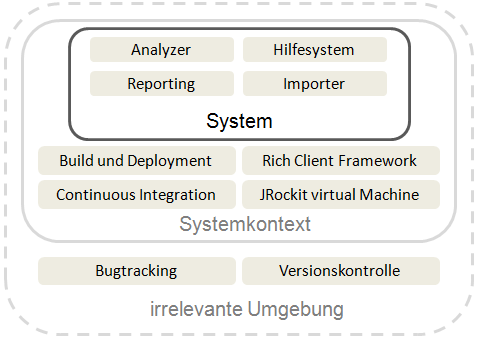
\includegraphics{images/systemumfang}
        	\caption{System und Systemkontext}
\end{figure}
\subsubsection{System}
Das System besteht aus den Teilen Datenmodell, Domäne, Log Parsing, Garbage Collection Analyse, Report, Charting, Hilfesystem\footnote{Dem Benutzer wird sowohl eine generelle wie auch eine kontextbezogene Hilfe angeboten.}, Benutzerführung.

\subsubsection{Systemkontext}
Zum Systemkontext gehören folgende nicht veränderbare Komponenten:
\begin{itemize}
	\item \textbf{Build und Deployment, Continuous Integration:} Der Build der Software für neue Updates oder Releases wird zentral auf einem Server durchgeführt. Der Source-Code wird aus der Versionskontrolle ausgecheckt, die binären Packete werden gebildet, es wird ein für den jeweiligen Update-Mechanismus notwendiges Packet erstellt und auf den Update-Server gestellt.

	\item \textbf{Update Mechanismus:} Die Software wird in der Version 1.0 released. Anschliessend können Updates (Minor-, Major-Versionen) direkt - ohne den manuellen Download der Software - durchgeführt werden.
	\item \textbf{JRockit Virtual Machine:} Die Schnittstelle zur JRockit Virtual Machine findet über deren Logdateien statt. Die genaurere Beschreibung befindet sich unter \titleref{jrockitgclog}.
\end{itemize}

\subsubsection{Irrelevante Umgebung}
\begin{itemize}
	\item \textbf{Issuetracker:} Sobald die Software stabil läuft und an Tester herausgegeben wird, wird für die Verwaltung der Fehler (Bugs) und Features ein Issuetracker verwendet.
	\item \textbf{Versionskontrolle:} Der Source-Code der Applikation wird in einer Source-Code-Verwaltung abgelegt. Diese dient als Backup und zur Versionierung der einzelnen Artefakte. Die beiden Werkzeuge (Issuetracker, Versionskontrolle) arbeiten normalerweise eng zusammen, so dass Bug Fixes mit der eingecheckten Version in Verbindung bleiben.
\end{itemize}


\subsection{Stakeholder}
Für die Anforderungsanalyse sind nur die mit Asteriks gekennzeichneten Stakeholder-Rollen relevant. Die anderen Rollen können erst dann berücksichtigt werden, wenn die Software eine weitere Verbreitung wahrnehmen kann. Verschiedene Rollen können auch von einer Person wahrgenommen werden. 
\begin{figure}[H]
  	\centering
    	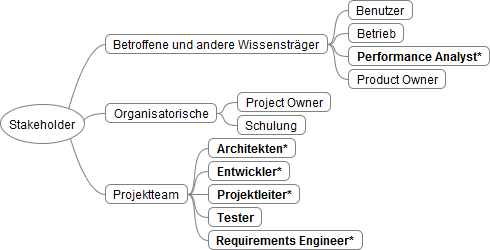
\includegraphics[width=13cm]{images/stakeholder_analyse}
        	\caption{Übersicht der Stakeholder}
\end{figure}

\subsection{Glossar}
Das Glossar befindet sich im Abschnitt \ref{glossar}. 
\subsection{Referenzen}
Die Referenzen innerhalb des Abschnitts \ref{anforderungsanalyse} befinden sich im Abschnitt Literaturverzeichnis.
\subsection{Übersicht}
Die Anforderungsanalyse ist folgendermassen aufgebaut: Beginnen tut sie mit der Allgemeinen Übersicht. Hier sind Architektur, Nutzer- und Zielgruppen, Randbedingungen und Annahmen dokumentiert. Danach sind die Anforderungen an die Software definiert, aus welchen sich anschliessend die unterschiedlichen Use Cases ableiten.
\section{Allgemeine Übersicht}\label{allgemeine_uebersicht}
\subsection{Architekturbeschreibung}
Die Software wird als Plugin programmiert. Der Entwickler kann sich die Software als Erweiterung in seiner Entwicklungsumgebung installieren. Sobald die Software installiert ist, wird für die Arbeit keine Verbindung ins Internet mehr benötigt. Die Applikation ist auf allen gängigen Betriebssystemen (Linux, Mac OSX, Windows) lauffähig.

\subsection{Nutzer und Zielgruppen}
\subsubsection{Performance Engineers}
Normalerweise Software Entwickler die viel Erfahrung, Wissen, Fähigkeiten haben und über die entsprechenden Werkzeuge verfügen, um die Ursachen für Performance-Probleme zu finden. Dabei handelt es sich nicht nur um Wissen im Bereich der Softwareentwicklung, sondern auch im Bereich des Servers und des Betriebssystems (Speichermanagement, I/O, etc.). Durch ihr breites Wissen sind sie mit der Unterstützung von Charts, Statistiken und Reports schnell in der Lage, Ursache von Performanceproblemen zu finden.

\subsubsection{Java Entwickler}
Im Gegensatz zu Performance Engineers beschäftigen sich Java Entwickler vorallem mit der Entwicklung von Anwendungen und verfügen nicht direkt über Knowhow im Bereich der Performanceanalyse. Als gut ausgebildete Ingenieure sind sie aber mit Hilfe von Werkzeugen und Dokumentation in der Lage, Performance Problemen innert nützlicher First auf den Grund zu gehen.

\subsection{Randbedingungen}\label{randbedingungen}
\subsubsection{JRockit R28}
Der Fokus der Analysesoftware stützt sich auf die Logdateien der JRockit Virtual Machine Release 28. Auswertungen der Garbage Collection von VMs anderer Hersteller werden höchstens zu einem späteren Zeitpunkt implementiert. 

\section{Use Cases}\label{use_cases}
Dieser Abschnitt zeigt die Use Cases für die Analysesoftware. Daraus werden dann im nächsten Abschnitt die Anforderungen respektive die finale Anforderungsliste abgeleitet. Als Einstieg dient das UML Use Case Diagramm, in welchem die Systemgrenzen, der Anwender (Performance Analyst) und die verschiedenen Use Cases dargestellt sind. Die einzelnen Use Cases sind dann nach der in \cite[S. 78-79]{pohl2010basiswissen} beschriebenen Schablone definiert.
\subsection{Übersicht}\label{systemfunktionalitaet}
 \begin{figure}[H]
  	\centering
    	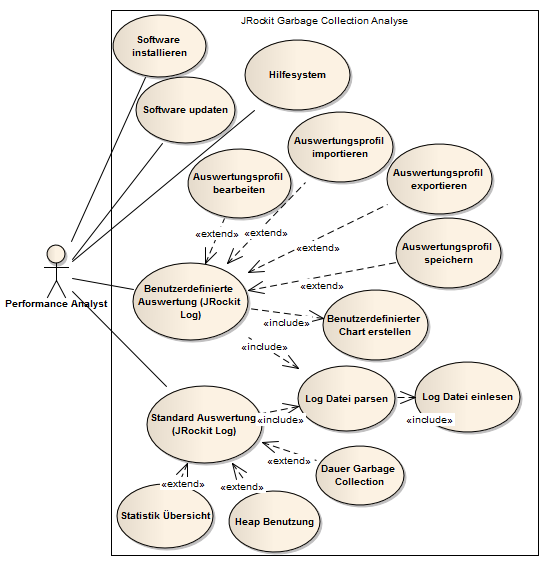
\includegraphics[width=14cm]{images/anforderungen_use-case}
        	\caption{Systemfunktionalität als Use-Case-Diagramm}
\end{figure}
\subsection{Beschreibung}
Die definierten Use Cases leiten sich aus einer Anforderung ab, welche über die Nummer referenziert ist.
\begin{longtable}{|p{4cm}|p{10.5cm}|}
  \hline
   \textbf{Abschnitt} & \textbf{Inhalt / Erläuterung} \\\hline
   Bezeichner & UC-01\\\hline
   Name & Software installieren\\\hline
   Autoren & Raffael Schmid\\\hline
   Priorität & Wichtigkeit für Systemerfolg: gross\newline Technologisches Risiko: mittel\\\hline
   Kritikalität & gross\\\hline
   Verantwortlicher & Raffael Schmid\\\hline
   Kurzbeschreibung & Der Benutzer kann die Software in seiner Entwicklungsumgebung installieren.\\\hline
   Akteure & Anwender, Entwicklungsumgebung\\\hline
   Auslösendes Ereignis & Anwender möchte eine Garbage Collection Logdatei analysieren.\\\hline
   Vorbedingung & Richtige Entwicklungsumgebung ist bereits ohne Analysesoftware installiert.\\\hline
   Nachbedingung & Es sind keine Fehler aufgetreten.\\\hline
   Ergebnis & Entwicklungsumgebung ist bereit für Garbage Collection Auswertungen.\\\hline
   Hauptszenario & 
         \begin{enumerate}
		\item Anwender Startet Entwicklungsumgebung
		\item Anwender gibt Update-Seite an
		\item Anwender selektiert zu installierendes Softwarepaket
		\item Softwarepaket wird installiert	
 	\end{enumerate}
	\\\hline
   Alternativszenarien & -\\\hline
   Ausnahmeszenarien & -\\\hline
   Qualitäten & Usability\\\hline
\caption{Use-Case: Software installieren}
\end{longtable}

\begin{longtable}{|p{4cm}|p{10.5cm}|}
\hline
   \textbf{Abschnitt} & \textbf{Inhalt / Erläuterung} \\\hline
   Bezeichner & UC-02\\\hline
   Name & Software updaten\\\hline
   Autoren & Raffael Schmid\\\hline
   Priorität & Wichtigkeit für Systemerfolg: gross\newline Technologisches Risiko: mittel\\\hline
   Kritikalität & Mittel\\\hline
   Verantwortlicher & Raffael Schmid\\\hline
   Kurzbeschreibung & Der Benutzer kann die Software updaten.\\\hline
   Akteure & Anwender, Update-Server\\\hline   
   Auslösendes Ereignis & Anwender hat die Software bereits zu einem früheren Zeitpunkt installiert. Sofern ein neues Update vorhanden ist, möchte er dieses installieren.\\\hline
   Vorbedingung & Richtige Entwicklungsumgebung und Software wurden bereits in einer früheren Version installiert.\\\hline
   Nachbedingung & Es sind keine Fehler aufgetreten.\\\hline
   Ergebnis & Entwicklungsumgebung und Analysesoftware sind auf dem neusten Stand für Garbage Collection Auswertungen.\\\hline
   Hauptszenario & 
	\begin{enumerate}
		\item Anwender Startet Entwicklungsumgebung
		\item Anwender sucht und findet Updates für die Analysesoftware
		\item Anwender selektiert eines oder mehrere dieser Softwarepakete
		\item Software wird aktualisiert
	\end{enumerate}
	\\\hline
   Alternativszenarien & -\\\hline
   Ausnahmeszenarien & -\\\hline
   Qualitäten & Usability\\\hline
\caption{Use-Case: Software updaten}
\end{longtable}

\begin{longtable}{|p{4cm}|p{10.5cm}|}
\hline
   \textbf{Abschnitt} & \textbf{Inhalt / Erläuterung} \\\hline
   Bezeichner & UC-03\\\hline
   Name & Garbage Collection Logdatei importieren\\\hline
   Autoren & Raffael Schmid\\\hline
   Priorität & Wichtigkeit für Systemerfolg: gross\newline Technologisches Risiko: gering\\\hline
   Kritikalität & gross\\\hline
   Verantwortlicher & Raffael Schmid\\\hline
   Kurzbeschreibung & Der Benutzer importiert die sich auf dem Dateisystem befindende Logdatei.\\\hline
   Akteure & Anwender, Logdatei Importer\\\hline
   Auslösendes Ereignis & Anwender startet Garbage Collection Log Analyse\\\hline
   Vorbedingung & Logdatei befindet sich auf dem Rechner und ist in einem der unterstützten Formate. Die Software ist vollständig installiert und gestartet.\\\hline
   Nachbedingung & Es sind keine Fehler aufgetreten. \\\hline
   Ergebnis & Die Logdatei ist in der Ansicht Logdateien ersichtlich und kann von da im Analysefenster geöffnet werden.\\\hline
   Hauptszenario & 
	\begin{enumerate}
		\item Anwender öffnet Import-Wizard
		\item Anwender navigiert zum Ordner
		\item Anwender selektiert Datei(en) und importiert diese
	\end{enumerate}
Die importierten Dateien werden gespeichert. Bei einem Neustart der Entwicklungsumgebung bleiben die zuvor importierten Dateien erhalten.
	\\\hline
   Alternativszenarien & -\\\hline
   Ausnahmeszenarien & -\\\hline
   Qualitäten & Usability\\\hline
\caption{Use-Case: Garbage Collection Logdatei importieren}
\end{longtable}

\begin{longtable}{|p{4cm}|p{10.5cm}|}
\hline
   \textbf{Abschnitt} & \textbf{Inhalt / Erläuterung} \\\hline
   Bezeichner & UC-04\\\hline
   Name & Standardauswertung anzeigen\\\hline
   Autoren & Raffael Schmid\\\hline
   Priorität & Wichtigkeit für Systemerfolg: gross\newline Technologisches Risiko: gross\\\hline
   Kritikalität & gross\\\hline
   Verantwortlicher & Raffael Schmid\\\hline
   Kurzbeschreibung & Für eine schnelle Übersicht steht eine Standard-Auswertung zur Verfügung. Diese soll eine kurze Übersicht über die Garbage Collection geben und beinhaltet zwei Charts (Heap Benutzung, Dauer Garbage Collection). \\\hline
   Akteure & Anwender, Logdatei Analyzer, Report Engine\\\hline
   Auslösendes Ereignis & Der Benutzer hat eine Garbage Collection Logdatei importiert und möchte nun die Analyse starten.\\\hline
   Vorbedingung & Bevor das Analysefenster für die Garbage Collection Logdatei geöffnet werden kann, wird die Datei eingelesen und geparst. Das heisst, dass die rohen Daten semantisch und syntaktisch analysiert und in den Arbeitsspeicher geladen werden.\\\hline
   Nachbedingung & -\\\hline
   Ergebnis & Dem Benutzer wird ein Analyse-Screen angezeigt.\\\hline
   Hauptszenario & 
	\begin{enumerate}
		\item Applikation hat die Logdatei fertig importiert.
		\item Dem Benutzer wird ein Screen mit verschiedenen Tabs angezeigt. Auf jedem Tab wird dem Benutzer eine unterschiedliche Sicht auf die Daten gezeigt.
	\end{enumerate}
	\\\hline
   Alternativszenarien & Benutzerdefinierte Auswertung\\\hline
   Ausnahmeszenarien & -\\\hline
   Qualitäten &  Korrektheit, Performance, Usability\\\hline
   Erweiterungen & UC-04.1, UC-04.2, UC-04.3, UC-04.4 \\\hline
\caption{Use-Case: Standardausertung anzeigen}
\end{longtable}

\begin{longtable}{|p{4cm}|p{10.5cm}|}
\hline
   \textbf{Abschnitt} & \textbf{Inhalt / Erläuterung} \\\hline
   Bezeichner & UC-04.1\\\hline
   Name & Anzeige Statistik Übersicht\\\hline
   Autoren & Raffael Schmid\\\hline
   Priorität & Wichtigkeit für Systemerfolg: gross\newline Technologisches Risiko: gross\\\hline
   Kritikalität & gross\\\hline
   Verantwortlicher & Raffael Schmid\\\hline
   Kurzbeschreibung & Der Analyse-Screen wurde geöffnet, dem Benutzer zeigen sich unterschiedliche Tabs. Auf dem ersten befinden sich verschiedene statistische Auswertungen der Logdatei:
   \begin{itemize}
	\item Übersicht und Grösse der verschiedenen Bereiche auf dem Heap: Initiale Grösse, endgültige Grösse
	\item Aktivitäten des Garbage Collectors: Anzahl Young Collections, Anzahl Old Collections
	\item Anzahl Garbage Collector Events (Bsp: Wechsel der Garbage Collection Strategie, etc.)
	\item Garbage Collection Zeiten (Total, Durchschnittliche, Zeit in Old Generation Garbage Collection, Prozentuale Zeit in Old Generation Garbage Collection)
	\item Durchsatz (siehe Abschnitt \ref{gc_tuning_durchsatz})
   \end{itemize}
 \\\hline
   Qualitäten &  Korrektheit, Performance, Usability\\\hline
\caption{Use-Case: Anzeige Statistik Übersicht}
\end{longtable}

\begin{longtable}{|p{4cm}|p{10.5cm}|}
\hline
   \textbf{Abschnitt} & \textbf{Inhalt / Erläuterung} \\\hline
   Bezeichner & UC-04.2\\\hline
   Name & Anzeige Heap Benutzung\\\hline
   Autoren & Raffael Schmid\\\hline
   Priorität & Wichtigkeit für Systemerfolg: gross\newline Technologisches Risiko: gross\\\hline
   Kritikalität & gross\\\hline
   Verantwortlicher & Raffael Schmid\\\hline
   Kurzbeschreibung & Die Heap Usage (Heap Benutzung) zeigt dem Benutzer anhand einer Grafik, zu welchem Zeitpunkt wieviel Speicher des Heaps verwendet wurde. Zusätzlich werden die Zeitpunkte inklusive entsprechendem Typ (Old- / Young-Collection) der Garbage Collection angezeigt.  \\\hline
   Qualitäten & Korrektheit, Performance, Usability\\\hline
\caption{Use-Case: Anzeige Heap Benutzung}
\end{longtable}

\begin{longtable}{|p{4cm}|p{10.5cm}|}
\hline
   \textbf{Abschnitt} & \textbf{Inhalt / Erläuterung} \\\hline
   Bezeichner & UC-04.3\\\hline
   Name & Anzeige Dauer Garbage Collection\\\hline
   Autoren & Raffael Schmid\\\hline
   Priorität & Wichtigkeit für Systemerfolg: mittel\newline Technologisches Risiko: mittel\\\hline
   Kritikalität & Mittel\\\hline
   Verantwortlicher & Raffael Schmid\\\hline
   Kurzbeschreibung & Für jede Garbage Collection ist innerhalb der Logdatei einen Eintrag mit den Informationen, wie viel Speicher von toten Objekten befreit wurde und wie lange die Collection gedauert hat. In diesem Report geht es um die Darstellung dieser Daten.\\\hline
   Qualitäten &  Korrektheit, Performance, Usability\\\hline
\caption{Use-Case: Anzeige Dauer Garbage Collection}
\end{longtable}

\begin{longtable}{|p{4cm}|p{10.5cm}|}
\hline
   \textbf{Abschnitt} & \textbf{Inhalt / Erläuterung} \\\hline
   Bezeichner & UC-05\\\hline
   Name &Profil (benutzerdefinierte Auswertung) erstellen\\\hline
   Autoren & Raffael Schmid\\\hline
   Priorität & Wichtigkeit für Systemerfolg: niedrig\newline Technologisches Risiko: niedrig\\\hline
   Kritikalität & Niedrig\\\hline
   Verantwortlicher & Raffael Schmid\\\hline
   Kurzbeschreibung & Der Benutzer kann ein eigenes Profil erstellen. Dem Profil können eigene, benutzerdefinierte Charts hinzugefügt werden. Auf jedem Chart können unterschiedliche Serien\footnote{Eine Serie definiert welche Daten auf der X- respektive Y-Achse angezeigt werden sollen.} hinzugefügt werden. Die Profile sind persistent und können exportiert wie auch importiert werden.\\\hline
   Akteure & Anwender, Logdatei Analyzer, Report Engine\\\hline
   Auslösendes Ereignis & Die Applikation hat die Datei fertig eingelesen und geparst.\\\hline
   Vorbedingung & Die Logdatei wurde ohne Fehler eingelesen und befindet sich im strukturierten Format im Arbeitsspeicher.\\\hline
   Nachbedingung & -\\\hline
   Ergebnis & Dem Benutzer wird ein benutzerdefiniertes Analysefenster angezeigt.\\\hline
   Hauptszenario & Unabhängig vom Zyklus der Garbage Collection Analyse, kann der Benutzer ein eigenes Profil erstellen. Ein Profil besteht initial aus einem Übersichtsfenster der Garbage Collection und kann um eigene, benutzerdefinierte Charts erweitert werden. Sollte die Entwicklungsumgebung mit der Analysesoftware geschlossen werden, bleiben die erstellten Profile erhalten.\\\hline
   Alternativszenarien & -\\\hline
   Ausnahmeszenarien & -\\\hline
   Qualitäten & Korrektheit \\\hline
\caption{Use-Case: Profil (benutzerdefinierte Auswertung) erstellen }
\end{longtable}




\begin{longtable}{|p{4cm}|p{10.5cm}|}
\hline
   \textbf{Abschnitt} & \textbf{Inhalt / Erläuterung} \\\hline
   Bezeichner & UC-6\\\hline
   Name & Hilfesystem\\\hline
   Autoren & Raffael Schmid\\\hline
   Priorität & Wichtigkeit für Systemerfolg: niedrig\newline Technologisches Risiko: mittel\\\hline
   Kritikalität & Mittel\\\hline
   Verantwortlicher & Raffael Schmid\\\hline
   Kurzbeschreibung & Dem Benutzer steht eine eine indexbasierte\footnote{Generelle Hilfe mit Informationen zur Garbage Collection,Vorgehensweise bei Performance Problemen, alternative Werkzeuge, etc.} und eine kontextsensitive\footnote{Hilfe zur aktuellen View oder Aktion des Benutzers} Hilfe zur Verfügung. \\\hline
   Akteure & Anwender\\\hline
   Auslösendes Ereignis & Anwender hat Plugin installiert, weiss nicht wie eine Analyse gestartet werden kann.\\\hline
   Vorbedingung & Entwicklungsumgebung und Software sind installiert.\\\hline
   Nachbedingung & -\\\hline
   Ergebnis & Anwender kennt Software\\\hline
   Hauptszenario &	\begin{itemize}
		\item \textbf{Indexbasierte Hilfe: } Der Benutzer kennt sich im Thema Garbage Collection und auf der Analysesoftware noch nicht aus. Er holt sich Hilfe über die indexbasierte Hilfe. 
		\item \textbf{Kontextsensitive Hilfe: } Der Benutzer befindet sich in einem Fenster oder möchte eine Aktion ausführen (Context), das Hilfesystem zeigt ihm dazu die notwendingen Informationen.
	\end{itemize}
	\\\hline
   Alternativszenarien & -\\\hline
   Ausnahmeszenarien & -\\\hline
   Qualitäten & Internationalisierung, Usability\\\hline
\caption{Use-Case: Hilfesystem}
\end{longtable}


\begin{landscape}
\section{Funktionale Anforderungen}
Aus den im Abschnitt \titleref{use_cases} definierten Anforderungen ergibt sich die abschliessende Liste der funktionalen Anforderungen:
\begin{longtable}{|p{1.8cm}|p{0.7cm}|p{2.5cm}|p{5cm}|p{1.6cm}|p{4cm}|p{0.9cm}|}
    \hline
   \textbf{Identifik.} & \textbf{Vers.}& \textbf{Titel} & \textbf{Beschreibung} & \textbf{Use Case} & \textbf{Abnahmekriter.} &\textbf{Prio.}\\\hline

   FRQ-01 & 1.0 & Installation & Software muss als Erweiterung in der Entwicklungsumgebung\footnote{Die Wahl der Entwicklungsumgebung respektive des Frameworks befindet sich im Abschnitt \titleref{selection_rcp_fw}.} installiert werden können.  & UC-01 & Entwickler mit durchschnittlichen Kenntnissen benötigen für die Installation in eine bestehende Entwicklungsumgebung dauert weniger als 5 Minuten. & gross  \\\hline

   FRQ-02 & 1.0 & Updaten & Die Software kann mit geringem Aufwand aktualisiert werden. & UC-02 & Entwickler mit durchschnittlichen Kenntnissen für den Update weniger als 3 Minuten. & mittel  \\\hline

  FRQ-03 & 1.0 & Garbage Collection Logdatei importieren & Logdateien können importiert werden und werden anschliessend in einem Fenster dargestellt. & UC-03 & - & gross  \\\hline

 FRQ-03.1 & 1.0 & Importierte Dateien speichern & Informationen über importierte Logdateien werden gespeichert und bleiben über die Zeit der Benutzersession bestehen.& UC-03.1 & - & gross  \\\hline

  FRQ-04 & 1.0 & Garbage Collection Logdatei einlesen & Geöffnete Garbage Collection Logdateien werden ins Memory gelesen. & UC-04 & Der Einleseprozess bei einer Datei mit 100000 Zeilen dauert weniger als 2 Sekunden. & gross  \\\hline

  FRQ-05 & 1.0 & Garbage Collection Logdatei parsen & Die eingelesenen JRockit Garbage Collection Logdatei wird geparst. Aus den Daten wird ein Domänenmodell aufgebaut.& UC-05 & Das Parsen einer Logdatei mit 100000 Zeilen dauert nicht länger als 8 Sekunden. & gross  \\\hline

   FRQ-06 & 1.0 & Standardauswert-ung anzeigen & Der Benutzer kann eine vordefinierte Anzeige öffnen. & UC-06 & - & gross \\\hline

   FRQ-06.1 & 1.0 & Anzeige Übersicht Garbage Collection & Der erste Tab des Analysefensters zeigt die aggregierten Daten der Garbage Collection. & UC-06.1 & Die Genauigkeit der berechneten und angezeigten Werte ist mindestens ein Zehntel (0.1). & gross \\\hline

   FRQ-06.2 & 1.0 & Anzeige Heap Benutzung & Der zweite Tab des Analysefensters zeigt den Speicherbedarf über die Zeit. & UC-06.2 & Die Genauigkeit der berechneten und angezeigten Werte ist mindestens ein Zehntel (0.1). & gross 
 \\\hline

   FRQ-06.3 & 1.0 & Anzeige Dauer Garbage Collection & Der dritte Tab des Analysefensters zeigt die Dauer der einzelnen Garbage Collections über die Zeit. & UC-06.3 & Die Genauigkeit der berechneten und angezeigten Werte ist mindestens ein Zehntel (0.1). & mittel 
 \\\hline

   FRQ-07 & 1.0 & Profil (Benutzerdefinierte Auswertung) erstellen & Benutzer kann Profil erstellen, um anschliessend darin benutzerdefinierte Charts zu erstellen.& UC-B07 & - & klein \\\hline

   FRQ-07.1 & 1.0 & Chart definieren für Profil & Für ein erstelltes Profil kann der Benutzer aus den Log-Daten ein eigenes Chart definieren. & UC-B07.1 & - & klein \\\hline

   FRQ-07.2 & 1.0 & Profil speichern & Definiertes Profil wird automatisch gespeichert und bleibt über die Dauer der Sitzung bestehen. & UC-07.2 & - & klein \\\hline

  FRQ-07.3 & 1.0 & Profil exportieren & Profil kann in Textdatei exportiert werden. & UC-07.3 & - & klein \\\hline

  FRQ-07.4 & 1.0 & Profil importieren & Profil kann aus Textdatei importiert werden. & UC-07.4 & - & klein \\\hline

  FRQ-08 & 1.0 & Hilfesystem &  Dem Benutzer werden eine indexbasierte und eine kontextsensitive Hilfe zur Verfügung gestellt. & UC-08 & Die Hilfe ist in Deutsch und Englisch verfügbar. & klein \\\hline
\caption{Funktionale Anforderungen}
\end{longtable}
\end{landscape}

\begin{landscape}
\section{Qualitätsanforderungen}
\subsection{Software}
\begin{longtable}{|p{1.8cm}|p{0.7cm}|p{2.5cm}|p{7cm}|p{4cm}|p{0.9cm}|}
    \hline
   \textbf{Identifik.} & \textbf{Vers.}& \textbf{Titel} & \textbf{Beschreibung} & \textbf{Abnahmekriter.} &\textbf{Prio.}\\\hline
   QRQ-S-01 & 1.0 & Erweiterbarkeit & Nebst der Analyse von Garbage Collection Logs der JRockit Virtual Machine sollen später auch andere Formate unterstützt sein. & Erweiterung um ein weiteres Logformat soll den Aufwand von 5 PT\footnote{Personentage} nicht überschreiten. & mittel \\\hline
   QRQ-S-02 & 1.0 & Testabdeckung & Um den langfristigen Erfolg dieser Software zu gewährleisten muss eine entsprechende Testabdeckung vorhanden sein - dies um insbesondere die Regression zu vermeiden. & Angestrebte Test-Coverage: 80\% & klein \\\hline
  QRQ-S-03 & 1.0 & Internationali-sierung & Die Sprachelemente der Software (Labels, Titel, Texte) werden als Ressourcen definiert, was die spätere Erweiterung ermöglicht. & - & klein\\\hline

   QRQ-S-04 & 1.0 & Usability & Schnelles Einlesen von grossen Dateien, Benutzerfeedback über ein Progressbar (Monitor).  & Der Import einer Log-Datei von 100000 Zeilen dauert kürzer als 10 Sekunden. Dem Benutzer wird ein Monitor bereitgestellt.&mittel \\\hline

  QRQ-S-05 & 1.0 & Korrektheit (angezeigte Werte) & Die berechneten und angezeigten Werte sind exakt. & berechnete und angezeigte Werte haben eine Genauigkeit von mindestens einem Zehntel (0.1). & gross\\\hline
\end{longtable}
\subsection{Basisframework}\label{anforderungen_framework}
\begin{longtable}{|p{1.8cm}|p{0.7cm}|p{2.5cm}|p{7cm}|p{4cm}|p{0.9cm}|}\hline
   \textbf{Identifik.} & \textbf{Vers.}& \textbf{Titel} & \textbf{Beschreibung} & \textbf{Abnahmekriter.} &\textbf{Prio.}\\\hline
   QRQ-F-01 & 1.0 & Verbreitung & Die Software wird als Erweiterung für eine Entwicklungsumgebung bereitgestellt. Die Verbreitung der Software spielt eine grosse Rolle.   & - & gross \\\hline

   QRQ-F-02 & 1.0 & Plattform-unabhängig & Software soll auf den gängigsten Betriebssystemen Windows und Apple OSX laufen. &  Framework läuft auf den Plattformen Windows und Mac OSX. & gross \\\hline

   QRQ-F-03 & 1.0 & Lokalisation & Framework muss Unterstützung für Lokalisation bereitstellen. & Framework bietet Unterstützung für die Mehrsprachigkeit. &klein \\\hline

   QRQ-F-04 & 1.0 & Modularisierung & Framework muss Unterstützung für Modularisierung bieten, damit die Software in unterschiedliche Komponenten aufgeteilt werden kann (siehe Erweiterbarkeit QRQ-S-01). & Framework bietet Unterstützung für Modularisierung.&mittel \\\hline

   FRQ-F-05 & 1.0 & Offline Betriebsmodus & Der Anwender soll die Software auch im Offline-Modus\footnote{Auf einem Computer der sich nicht am Netz befindet.} benutzen können. & Eigenständige Software, keine Web Applikation & gross  \\\hline

   FRQ-F-06 & 1.0 & Installation als Erweiterung& Software wird als Erweiterung in einer Entwicklungsumgebung installiert. & - & gross  \\\hline

    \caption{Qualitätsanforderungen Basisframework}
\end{longtable}
\end{landscape}





\part{Konzept}
\chapter{Auswahl Frameworks und Komponenten}\label{selection_rcp_fw}
Im Vorfeld des Software-Konzepts wird die Evaluation der verschiedenen Rich Client Frameworks durchgeführt. Dieser Abschnitt beinhaltet sowohl die ''Analyse über Stärken und Schwächen der bestehenden Java Rich Client Technologien`` als auch die ''dokumentierten Auswahlkriterien und Entscheidungsgrundlagen``. Der Abschnitt besteht aus drei Teilen: der erste Teil beschreibt das Bewertungsschema, der zweite und dritte die Evaluation von Rich Client Framework und Charting Bibliothek.


\section{Bewertung}
Die Evaluation und Bewertung des Rich Client Frameworks und der Charting Bibliothek basiert auf dem nachfolgend beschriebenen Berechnungsmodell. 

Auf der Basis der Anforderungen werden die Bewertungskriterien definiert. Die Gewichtung leitet sich folgendermassen aus der Priorität ab:
\begin{longtable}{|l|c|c|c|c|c|}\hline
 \textbf{Priorität} & sehr klein & klein & mittel & gross & sehr gross\\\hline
 \textbf{Gewicht} & 1 & 2 & 3 & 4 & 5\\\hline
 \caption{Schema Umwandlung Priorität in Gewicht}
\end{longtable}

Die Bewertung der Komponenten hinsichtlich den Kriterien basiert auf dem aus der Evaluation erhaltenen Erfahrungswert und wird folgendermassen in eine Zahl umgewandelt:
\begin{longtable}{|l|c|c|c|c|c|}\hline
 \textbf{Bewertung} & sehr schlecht & schlecht & mittel & gross & sehr gross\\\hline
 \textbf{Zahl} & 1 & 2 & 3 & 4 & 5\\\hline
 \caption{Schema Vergabe der Punkte}
\end{longtable}

Die Punktezahl berechnet sich aus dem Produkt aus Gewichtung und Bewertung:
\begin{center}
\fbox{Punktezahl = Gewichtung x Bewertung}
\end{center}
\section{Evaluation Rich Client Framework}
Grundsätzlich kommen für die Entwicklung der Analysesoftware auch die Java GUI-Bibliothek Swing in Frage. Viele der Anforderung (Deployment, Installation, Update, Modularisierung, Internationalisierung, etc.) werden von Rich Client Frameworks bereitgestellt und stehen mit teilweise geringem Aufwand zur Verfügung. Bei der Evaluation der Bibliothek werden darum nur Rich Client Frameworks berücksichtigt. Von denen kommen aufgrund der funktionalen Anforderung QRQ-F-05 (Offline Betriebsmodus) und QRQ-F-06 (Installation als Erweiterung) Eclipse RCP und Netbeans RCP in Frage. Während Eclipse RCP insbesondere als Entwicklungsumgebung ein weit verbreitetes Framework ist und die Entwicklung aktuell in zwei verschiedenen Versionen (3.x / 4.x) vorangetrieben wird, findet man Netbeans und deren Rich Client Plattform eher selten. In der Folge werden die drei Frameworks kurz beschrieben und dann anhand der Anforderungen verglichen.


\subsection{Eclipse RCP}
Bis zur Version 2.1 war Eclipse bekannt als eine Open Source Entwicklungsumgebung für Programmierer. Der Vorgänger hiess Visual Age vor Java und wurde von IBM entwickelt. 

Auf die Version 3.0 wurde die Architektur von Eclipse relativ stark umgestellt und modularisiert. Seit dem handelt es sich um einen relativ kleinen Kern, der die eigentlichen Funktionalitäten der Applikation als Plugins lädt. Der beschriebene Mechanismus basiert auf Eclipse Equinox, einer Implementation der OSGi Spezifikation. Die grafischen Benutzeroberflächen werden in SWT implementiert. Die Plattform kann nun auch als Framework zur Entwicklung von Desktop Applikationen oder Plugins für die Entwicklungsumgebung  verwendet werden.

\begin{itemize}
\item \textbf{Verbreitung:} Eclipse RCP ist relativ stark verbreitet, die Suche auf Amazon nach "Eclipse RCP" (Kategorie: Bücher) liefert 53 Resultate (stand 27. November 2011).
\item \textbf{Plattformunabhängigkeit:} Eclipse ist für 14 verschiedene Systeme und Architekturen bereitgestellt und gilt somit als plattformunabhängig\cite{wiki:eclipse}.
\item \textbf{Lokalisation:} Wird von Eclipse unterstützt durch die Erweiterung der Java-Lokalisation.
\item \textbf{Modularisierung:} Die Modularisierung in Eclipse Anwendungen wird auf der Basis von Plugins gemacht. Ein Plugin ist eine Menge von Klassen mit einer wohl definierten Schnittstelle (welche Klassen, Packete werden importiert, exportiert).
\item \textbf{Installation als Erweiterung:} Eclipse bietet an, Plugins und Features in die bestehende Entwicklungsumgebung zu installieren.
\end{itemize}

\subsection{Netbeans RCP}
Bei Netbeans RCP handelt es sich ebenfalls um ein Framework zur Entwicklung von Desktop Anwendungen. Der Kern der Netbeans Plattform besteht ebenfalls aus einem Modul-Loader und im Bereich der grafischen Benutzeroberfläche wird Swing verwendet. 
\begin{itemize}
\item \textbf{Verbreitung:} Netbeans RCP ist nicht sehr verbreitet, die Suche auf Amazon nach "Netbeans RCP" (Kategorie: Bücher) liefert 7 Resultate (stand 27. November 2011).
\item \textbf{Plattformunabhängigkeit:} Netbeans RCP basiert vollumfänglich auf Java und ist deshalb auf allen Plattformen, für die eine Java Virtual Machine existiert, verfügbar. Es gilt deshalb als plattformunabhängig (siehe \cite{wiki:netbeans}).
\item \textbf{Lokalisation:} Wird von Netbeans unterstützt durch die Erweiterung der Java-Lokalisation.
\item \textbf{Modularisierung:} Die Modularisierung in Netbeans kann ebenfalls mit Modulen (äquivalent Plugin in Eclipse Applikationen) gemacht werden.
\item \textbf{Installation als Erweiterung:} Netbeans bietet es an, Module in die bestehende Entwicklungsumgebung zu installieren.
\end{itemize}

\subsection{Auswertung}
Die erste und zweite Spalte zeigen die Anforderungen aus Abschnitt \ref{anforderungen_framework}. Die dritte Spalte enthält das aus der Priorität abgeleitete Gewicht (siehe Abschnitt Gewichtung). Die weiteren Spalten zeigen pro Kandidat die Bewertung zusammen mit dem errechneten Produkt aus Gewichtung und Bewertung.
\begin{longtable}{|p{3cm}|c|c|c|c|c|}\hline
 \textbf{Anforderung\footnote{siehe Abschnitt \ref{anforderungen_framework}}} & \textbf{Nummer} &  \textbf{Gewicht.\footnote{Gemäss Priorität der Anforderung}} & \textbf{Eclipse 3.x} & \textbf{Eclipse 4.x} &  \textbf{Netbeans 3.x}\\\hline
   Verbreitung & (QRQ-F-01) & 4 & 5 (20) & 1 (4) & 2 (8)\\\hline
   Unterstützung Plattformunab-hängigkeit & (QRQ-F-02) & 4 & 5 (20) & 5 (20) & 5 (20)\\\hline
   Unterstützung Lokalisation Support & (QRQ-F-03) & 2 & 5 (10) & 5 (10) & 5 (10) \\\hline
   Unterstützung Modularisierung & (QRQ-F-04) & 3 & 5 (15) & 5 (15) & 5 (15) \\\hline
   Offline Betriebsmodus & (QRQ-F-05) & 4 & 5 (20) & 5 (20) & 5 (20) \\\hline
   Installation als Erweiterung & QRQ-F-06 & 4 & 5 (20) & 5 (20) & 5 (20) \\\hline
   \textbf{Total} & & & \textbf{105} & \textbf{89} & \textbf{93}\\\hline
    \caption{Auswertung Rich Client Frameworks}
\end{longtable}

Ausschlaggebend für die Wahl der Rich Client Plattform ist die Verbreitung. Trotz der Unterschiede in Architektur und den verwendeten Technologien sind sie hinsichtlich Funktionsumfang praktisch identisch. Laut \cite{toedter20071120} können häufig auftretende Use Cases an eine Rich Client Applikation sowohl mit der Netbeans als auch mit der Eclipse Plattform umgesetzt werden.


\section{Evaluation Bibliothek Charting}
Für die grafische Darstellung der Daten (Charts) muss eine Bibliothek verwendet werden. Im Bereich der nicht-kommerziellen Produkte wird dafür sehr oft Eclipse BIRT und JFreeChart eingesetzt.
\subsection{Business Intelligence and Reporting Tools (BIRT)}
BIRT steht für Business Intelligence and Reporting Tools und stellt Business-Intelligence- und Reporting-Funktionalität für Rich Clients zur Verfügung. BIRT ist Lizenziert unter der Eclipse Public License und ist daher open-source. BIRT ist wie Eclipse ein Top-Level-Softwareprojekt der Eclipse Foundation. Die Software besteht aus zwei Teilen:
\begin{itemize}
\item \textbf{Report Designer: }Mit dem Report Designer können Benutzer oder Administratoren ihre Reports erstellen und anpassen. 
\item \textbf{Charting Engine: }Die Charting Engine generiert aus den Daten und den definierten Reports, Diagrammen die Charts.
\end{itemize} 

Der Umfang der Software ist mit über 100 Megabyte für kleinere Projekte eher ungeeignet.

\subsection{JFreeChart}
JFreeChart ist ein Open-Source-Framework mit welchem eine Vielzahl verschiedener Diagramme erzeugt werden können. JFreeChart unterstützt die Ausgabe der Diagramme in Grafiken, Swing- und RCP-Applikationen und ist mit einer Grösse von rund einem Megabyte auch für kleinere Softwareprojekte geeignet.

\subsection{Auswertung}
\begin{longtable}{|p{4cm}|c|c|c|c|}\hline
 \textbf{Anforderung\footnote{Es wurden nur die für die Evaluation der Charting Bibliothek relevanten Anforderungen aus Abschnitt \ref{anforderungen_software} und \ref{anforderungen_framework} übernommen.}} & \textbf{Nummer} &  \textbf{Gewicht.\footnote{Gemäss Priorität der Anforderung}} & \textbf{BIRT} & \textbf{JFreeChart}\\\hline
   Grösse Softwarepacket & (QRQ-S-06) & 4 & 1 (4) & 5 (20) \\\hline
   Verbreitung & (QRQ-F-01) & 4 & 4 (16) & 5 (20) \\\hline
   \textbf{Total} & && \textbf{20}  & \textbf{40} \\\hline
    \caption{Auswertung Charting-Bibliothek}
\end{longtable}

\subsection{Entscheid}
JFreeChart eignet sich insbesondere für kleinere Client-Applikationen sehr gut zur Erstellung von Diagrammen. Die Flexibilität welche bei Birt durch den Report-Designer bereitgestellt wird, kann in der Analysesoftware nicht angewendet werden. Deshalb fiel der Entscheid für die Bibliothek JFreeChart aus.

\chapter{Architektur}\label{konzept_1}
Als Basis für die Konzeption der funktionalen Anforderungen wird in diesem Abschnitt die Architektur der Software definiert. Nebenbei befinden sich darin auch einige allgemeine Informationen wie beispielsweise das Thema der Lizenzierung.
\section{Allgemein}
\subsection{Ausgangslage}
Als Rich Client Framework wird Eclipse 3.x\footnote{die aktuelle Version ist 3.7 (stand: 31.8.2011)} genommen. Siehe Abschnitt \titleref{selection_rcp_fw}. In der Folge werden die für die Eclipse Plattform gebräuchlichen Begrifflichkeiten verwendet. 

\subsection{Lizenzierung der Software}
Die Software wird lizenziert unter der Eclipse Public License\footnote{http://www.eclipse.org/legal/epl-v10.html} in der Version 1.0. Dies ist eine freie Software-Lizenz und gewährt das Recht zur freien Nutzung, Weiterverbreitung und Veränderung der Software. Die Benutzung einer Open-Source Lizenz hat insbesondere folgende Vorteile:
\begin{itemize}
	\item An der Entwicklung von Open-Source Software können sich eine beliebige Anzahl an Entwickler beteiligen. Der Entwicklungsaufwand kann skaliert werden.
	\item Jedermann kann Erweiterungen entwickeln oder Fehler beheben.
\end{itemize}

\section{Übersicht}\label{konzept_uebersicht}
Aufgrund der Anforderung QRQ-S-01 (Erweiterbarkeit) muss die Analysesoftware auch hinsichtlich anderer Logformate erweiterbar sein. Die Applikation wird also nicht zwingendermassen mit der Erweiterung für JRockit Logdateien verwendet. Es könnte zu einem späteren Zeitpunkt sein, dass man damit Garbage Collection Logs der HotSpot virtual Machine auswertet. Dies hat hinsichtlich Architektur einige Konsequenzen:
\begin{itemize}
	\item Die Applikation wird in zwei Komponenten aufgeteilt:
		\begin{itemize}
			\item Basissoftware
			\item Erweiterung JRockit
		\end{itemize}
		Die Basissoftware kann unabhängig von den Erweiterungen installiert werden, für die Auswertung wird die entsprechende Erweiterung allerdings benötigt. Eine Erweiterung kann ohne Basissoftware nicht gebraucht werden.
	\item Die Architektur der Applikation muss es zulassen, dass zu einem späteren Zeitpunkt auch Garbage Collection Logs von anderen virtuellen Maschinen analysiert werden.
	\item Die Basissoftware stellt Extension-Points\footnote{Ein Extension-Point ist ein Mechanismus, mit dem zwei Eclipse-Plugins miteinander kommunizieren können.} bereit, über welche sich die Erweiterungen  registrieren.
\end{itemize}

\subsection{Struktur}\label{projektstruktur}
Die generischen Aspekte der Software befinden sich in der Basissoftware. Nur die Spezialisierung im Bereich jedes einzelnen Log-Formats findet in den Erweiterungen statt. Die Aufgaben werden folgendermassen verteilt:
\begin{itemize}
	\item Basissoftware (Core Feature)
		\begin{itemize}
			\item Garbage Collection Log importieren
			\item Garbage Collection Log einlesen
			\item Profil erstellen, speichern, exportieren, importieren
			\item Hilfesystem (wobei allerdings jedes einzelne Feature spezifische Hilfethemen bereitstellen kann)
		\end{itemize}
	\item JRockit Extension (JRockit Extension Feature)
		\begin{itemize}
			\item Garbage Collection Log parsen
			\item Jede Erweiterung hat ein eigenes Domänemodell, da der Aufbau des Garbage Collectors Herstellerabhängig ist.
		\end{itemize}
\end{itemize}

Das Core-Feature ist die Basis und verantwortlich für den gesamten Import-Prozess (Import-Wizard, Leseprozess der Log-Datei, Anzeige der Menus, Profil-Verwaltung, etc.). Die JRockit Extension ist eine für die Garbage Collection Logs der JRockit geschriebene Erweiterung. Sie ist für das Parsen der Logdateien sowie die Aufbereitung und das Bereitstellung der Daten zuständig. Beinhaltet aber keine Basisfunktionalität.
 \begin{figure}[H]
  	\centering
    	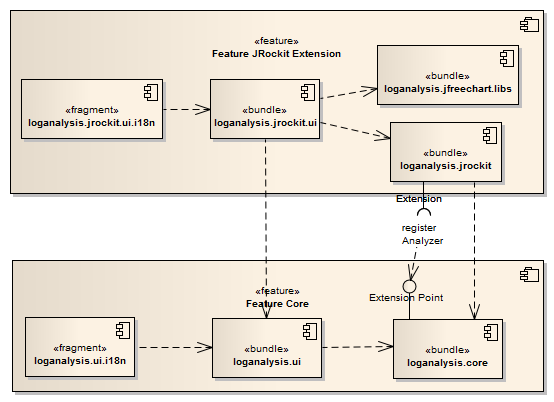
\includegraphics[width=14cm]{images/architektur_komponenten_uebersicht}
        	\caption{Architektur: Komponentendiagramm}
\end{figure}

Das Core Feature besteht aus dem Modul User Interface (``loganalysis.core.ui'') und einem von JFace und SWT\footnote{JFace und SWT wird in Eclipse als Library für die Präsentationsschicht verwendet.} unabhängigen Teil (``loganalysis.core''). Öffnet der Benutzer eine Garbage Collection Logdatei, wird diese durch das Core Feature eingelesen und der Inhalt wird an alle verfügbaren Extensions weitergeleitet. Die erste Extension welche den Inhalt der Datei verarbeiten kann, öffnet seine dafür vorgesehenen Reports und Charts. Jede Extension hat ein basierend auf der Logdatei eigenes Domänen-Modell.

\subsubsection{Nicht-funktionale Module}
Die folgenden Projekte (Plugins) sind im Zusammenhang mit dem Deployment und Testing notwendig, beinhalten aber keine eigentliche Funktionalität. In der Regel beinhalten sie Konfigurationsdateien oder Test-Klassen:
\begin{itemize}
	\item Test-Projekte\footnote{Der Test-Code befindet sich in eigenen Projekten (siehe Abschnit \ref{testing}).}
		\begin{itemize}
			\item core.test
			\item core.ui.test
			\item jrockit.test
			\item jrockit.ui.test
		\end{itemize}
	\item  Features\footnote{Features sind in sich lauffähige Softwarekomponenten mit definiertem Umfang und Abhängigkeiten auf Plugins. Zur Defininition wird ein eigenes Eclipse-Projekt erstellt.}
		\begin{itemize}
			\item loganalysis.feature
			\item loganalysis.jrockit.feature
		\end{itemize}
	\item  Thirdparty Bibliotheken\footnote{Eingebundene externe Bibliotheken werden als Plugins gepackt, damit deren Klassen durch den Modul-Loader geladen werden können.}
		\begin{itemize}
			\item  loganalysis.jfreechart.libs (JFreeChart Library)
		\end{itemize}
	\item  Targetplattform\footnote{Definiert gegen welche Plattform die Anwendung entwickelt wird.}
		\begin{itemize}
			\item  loganalysis.targetplatform (beinhaltet die Target-Plattform)
		\end{itemize}
	\item  Update-Seite\footnote{Definiert bereitgestellte Features}
		\begin{itemize}
			\item loganalysis.updatesite (definiert und generiert die Update-Seite)
		\end{itemize}
\end{itemize}



\chapter{Konzept funktionale Anforderungen}\label{konzept_2}
\section{Installation (FRQ-01)}\label{installation}
Zur Installation der Software benötigt man die Eclipse-Entwicklungsumgebung in der Version 3.7. Darin integriert befindet sich ein Update-Manager, der Software-Komponenten von Lokal oder dem Netzwerk installieren kann. Auch Updates werden über diesen Mechanismus installiert. Die Analysesoftware wird via eine Update-Seite bereitgestellt. Der Software-Build durch das Continuous Integration System publiziert die Artefakte (Features, Plugins) auf einen via Internet zugänglichen Server, von welchem der Update-Manager die Software herunterlädt um anschliessend zu importieren. Update-Seiten im Eclipse-Umfeld bestehen aus Features (Eclipse Feature-Projekt). Features bestehen aus unterschiedlichen Plugins (Eclipse Plugin-Projekt). Die Eclipse Runtime kann solche Softwarepakete zur Laufzeit installieren und updaten.

Die Update-Seite widerspiegelt die Struktur der Software:
\begin{itemize}
\item \textbf{Basissoftware:} Umfasst alle Plugins , die für die Basissoftware notwendig sind (Siehe Abschnitt \ref{projektstruktur}).
\item \textbf{JRockit Erweiterung: }Umfasst alle Plugins zur JRockit Erweiterung und hat zugleich die Abhängigkeit auf das Basissoftware-Feature.
\end{itemize}

\section{Update (FRQ-02)}
Der Update eines Features auf der Update-Seite durch die Erstellung eines neuen Releases ist erkennbar durch eine Änderung der Versionsnummer. Beim Starten der Software wird überprüft, ob ein sich auf dem Server befindendes Feature aktualisiert wurde. Der Benutzer kann diese im laufenden Betrieb der Applikation installieren, ein Neustart ist allerdings danach Pflicht.

\section{Datei importieren (FRQ-03)}
Der Import\footnote{Der Begriff Import ist irreführend, da diese Aktion einzig dazu dient, die Datei in die Ansicht Logdateien zu kriegen. Erst mit dem Öffnen der Datei werden die Daten wirklich gelesen.} einer Logdatei findet über einen Import-Wizard statt. Der Ablauf ist folgendermassen:
\begin{enumerate}
	\item Import-Wizard öffnen
	\item Auswahl des Ordners
	\item Selektion einer oder mehrerer Logdateien
	\item Bestätigung der Eingaben
	\item Anschliessend wird die Logdatei als Instanz von \textit{IFileDescriptor} in der Ansicht \textit{Logdateien} angezeigt, der Inhalt wurde allerdings noch nicht analysiert.
\end{enumerate}

\section{Importierte Dateien speichern (FRQ-04)}
Der im Abschnitt \ref{memento} beschriebene Mechanismus wird verwendet, damit nach einem Neustart der Entwicklungsumgebung die importierten Logdateien nicht verloren gehen. 

\section{Datei einlesen (FRQ-05)}
Durch den Import einer Garbage Collection Logdatei erscheinen diese im Fenster \textit{Logdateien}. Das öffnen einer dieser Dateien lädt den Inhalt in den Arbeitsspeicher. Die Daten sind noch unstrukturiert und werden innerhalb des im nächsten Abschnitt definierten Domänenmodells gespeichert.

\subsection{Domänenmodell}
\textit{IFileDescriptor} wird für die Abstraktion der Garbage Collection Logdatei verwendet. Darin enthalten sind Metadaten wie Dateiname und Pfad sowie - wenn bereits geladen - der Inhalt der Datei. Die Abstraktion einer Garbage Collection Logdatei heisst \textit{AbstractJvmRun} und wird erst von der jeweiligen Erweiterung realisiert.
 \begin{figure}[H]
  	\centering
    	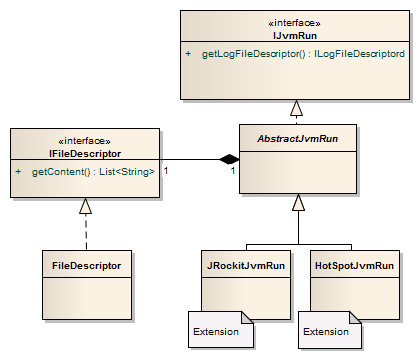
\includegraphics[width=16cm]{images/core_domain}
        	\caption{Domänenmodell: Eingelesene Datei}
\end{figure}

\section{Logdatei parsen (FRQ-06)}
Die Garbage Collection Logs der JRockit Virtual Machine bestehen aus Einträgen unterschiedlicher Log Module. Diese Ausgaben können selektiv per Kommandozeile aktiviert werden (siehe Abschnit \ref{logmodule}). Für die Garbage Collection Analyse sind nicht alle Einträge relevant, es werden nur die wichtigsten verwendet. Die einzelnen Parser für die Garbage Collection Logdatei werden auf der Basis von Regular Expressions selber implementiert. Auf die Verwendung eines Parser-Generators wird aus folgenden Gründen verzichtet:
\begin{itemize}
	\item Lightweight: Um Parser-Generatoren zu verwenden, wird in der Regel auch zur Laufzeit eine Bibliothek benötigt. Diese muss mit der Software ausgeliefert werden. Die Implementation eines Parser auf der Basis von Regulären Ausdrücken kann mit Java Standardmitteln gemacht werden.
	\item Proprietär: Parser-Generatoren sind proprietär und die Verwendung dessen bedingt gute Kenntnisse. In der Regel beschreibt man das Format in einer Grammatik.
\end{itemize}

\subsection{Parser}
Der Parser für die Logdateien der JRockit Virtual Machine ist nach dem Chain-of-Responsibility Pattern\cite{wiki:chainOfResponsibilityPattern} aufgebaut. Dieses Pattern ermöglicht die schnelle Erweiterbarkeit (Anforderung QRQ-S-01) der Software um weitere Parser. Pro Log-Eintrag (respektive pro Typ eines Log-Eintrags) kann ein Parser in die Parser-Kette geschaltet werde. Jeder Parser extrahiert die für ihn wichtigen Informationen und aktualisiert damit das Domänenmodell. Die wichtigsten Einträge der Garbage Collection Logdatei sind die des Memory Modules und werden vom \textit{MemoryModuleParser} verarbeitet. In zukünftigen Versionen ist die Verarbeitung von Log-Einträgen von anderen Log-Modulen denkbar - Einträge des Nursery- oder Allocation-Modules, etc. Ablauf und Aufbau des Parsers sind in den folgenden beiden Grafiken ersichtlich:

 \begin{figure}[H]
  	\centering
    	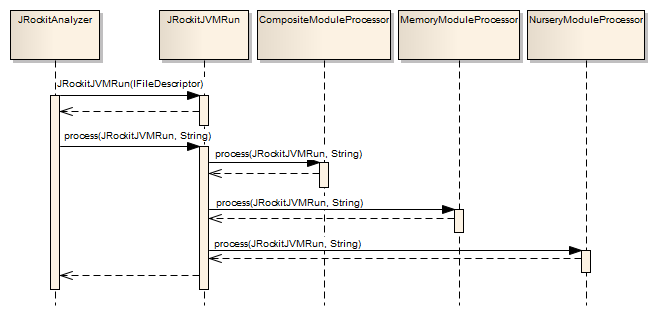
\includegraphics[width=16cm]{images/acitivity_parse_prozess}
        	\caption{Sequenzdiagramm Parser}
\end{figure}
 \begin{figure}[H]
  	\centering
    	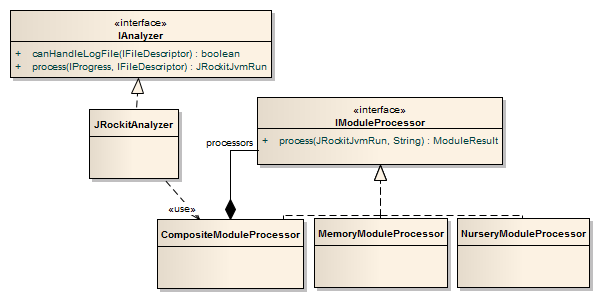
\includegraphics[width=16cm]{images/jrockit_log_processing}
        	\caption{Klassendiagramm Parser}
\end{figure}

\subsubsection{MemoryModuleParser}
Das Parsen innerhalb des \textit{MemoryModuleParser} wird in zwei Schritte aufgeteilt:
\begin{itemize}
\item \textbf{Lexer: }Der einzelne Logeintrag wird durch den Lexer (Tokenizer) in eine Map aus Tokens umgewandelt. Schlüssel für die einzelnen Tokens ist der \textit{TokenType}. Der Lexer wird mittels Regular Expressions implementiert. Die Werte werden mittels Gruppierungs-Funktion\footnote{Mittels Gruppen innerhalb von Regulären Ausdrücken lassen sich einzelne Werte aus einem String extrahieren.} extrahiert. 
\item \textbf{Syntactic Analyzer: }Der syntaktische Analyser verarbeitet die vom Lexer extrahierten Tokens. Er führt zum einen eine semantische Validierung durch und speichert die Werte in strukturierter Form (Domänenmodell).
\end{itemize}

\subsection{Auswertung Logdatei}
Bereits in Abschnitt \ref{logexample} ist ein Teil einer Garbage Collection Logdatei aufgelistet. Dieser Abschnitt zeigt die für die Garbage Collection Analyse wichtigsten Informationen und Auswertungen die mit der Analysesoftware dafür gemacht werden können, ohne dabei aber auf die Ausgaben des Debug-Log-Levels\footnote{Der Log-Level kann für jeden einzelnen Logger eingstellt werden.} einzugehen.

\subsubsection{Garbage Collection Algorithmus}
\begin{lstlisting}[numbers=none,  framexleftmargin=0mm, caption=Logdatei: Ausgabe initialer Garbage Collection Algorithmus]
[INFO ][memory ] GC mode: Garbage collection optimized for throughput, strategy: Generational Parallel Mark & Sweep.
\end{lstlisting}
Die eigentlich wichtigste Information respektive Entscheidung zum Garbage Collection Tuning ist die Wahl der Strategie. Sie wird im Header der Logdatei angezeigt und entspricht entweder der Standardeinstellung oder wird konfiguriert. Ausgewertet aus dem Eintrag werden zwei Dinge: für was die Garbage Collection optimiert ist (Durchsatz oder Pausenzeiten) und die Strategie (Generational Parallel Mark \& Sweep, Parallel Mark \& Sweep, Genertional Concurrent Mark \& Sweep, Concurrent Mark \& Sweep).
	
\subsubsection{Initiale und maximale Heap-Kapazität, Grösse Old- und Young-Space}
\begin{lstlisting}[numbers=none,  framexleftmargin=0mm, caption=Logdatei: Initiale und maximale Heap-Kapazität und Grösse des Old- und Young-Spaces]
[INFO ][memory ] Heap size: 65536KB, maximal heap size: 1048576KB, nursery size: 32768KB.
\end{lstlisting}
Ebenfalls im Header der Logdatei befindet sich die Angabe über die initiale und maximale Heap-Kapazität und die grösser des Young-Spaces (Nursery). Die grösse des Old-Spaces (Tenured Space) errechnet sich aus der Differenz zwischen Young-Space und maximaler Kapazität.

\subsubsection{Young-Collection Information}
\begin{lstlisting}[numbers=none,  framexleftmargin=0mm, caption=Logdatei: Information Young-Collection]
[INFO ][memory ] [YC#660] 2.172-2.172: YC 200108KB->200147KB (233624KB), 0.001 s, sum of pauses 0.536 ms, longest pause 0.536 ms.
\end{lstlisting}
Der Abschluss einer Young-Collection wird mit dem oben aufgelisteten Log-Eintrag dokumentiert. Er beschreibt Start- und Endzeitpunkt sowie die Grösse des Heaps vor und nach der Garbage Collection. Des weiteren ist die Dauer, die Summe aller einzelnen Pausen und die längste Pause aufgelistet. 

\subsubsection{Old-Collection Information}
\begin{lstlisting}[numbers=none,  framexleftmargin=0mm, caption=Logdatei: Information Old-Collection]
[INFO ][memory ] [OC#3] 2.544-2.733: OC 233624KB->187955KB (280628KB), 0.189 s, sum of pauses 187.019 ms, longest pause 187.019 ms.
\end{lstlisting}
Die Ausgabe einer Old-Collection unterscheidet sich, ausgenommen vom Typ (OC),  nicht von der einer Young-Collection.

\subsubsection{Wechsel der Garbage Collection Strategie}
\begin{lstlisting}[numbers=none,  framexleftmargin=0mm, caption=Logdatei: Wechsel Garbage Collection Strategie]
[INFO ][memory ] [OC#6] Changing GC strategy from: singleconpar to: singleconcon, reason: Return to basic strategy.
\end{lstlisting}
Aus unterschiedlichen Gründen kann es zu einem Wechsel der Garbage Collection Strategie kommen. Dieser wird, zusammen mit dem Grund für den Wechsel, in der Logdatei dokumentiert und kann ausgewertet werden.


\subsection{Domänenmodell JRockit Garbage Collection}\label{jrockit_domain_model}
Nach der syntaktischen und sematischen Analyse wird eine Instanz des Domänenmodells erzeugt. Dieses wurde aufgrund der Randbedingungen (siehe Abschnitt \ref{randbedingungen}) analog der Struktur der Garbage Collection in der JRockit Virtual Machine abstrahiert. Die rohen Daten sind also danach über dieses sich im Arbeitsspeicher befindende Objekt verfügbar. \begin{landscape}
 \begin{figure}[H]
  	\centering
        	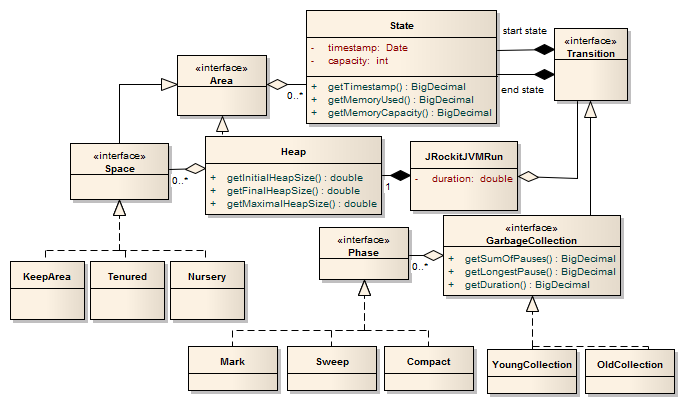
\includegraphics[width=18.2cm]{images/jrockit_extension_domain}
	\caption{Domänenmodell: Garbage Collection (JRockit Implementation)}
\end{figure}
\end{landscape}
Die Daten der Logdatei repräsentieren einen Lauf einer JVM (\textit{JRockitJVMRun}) bestehend aus einem Heap und den darin enthaltenen Bereichen Keep-Area, Nursery und Tenured Space. Jeder dieser Bereiche hat unterschiedliche Zustände (\textit{State}). Beim Übergang (\textit{Transition}) vom einen in den anderen Zustand findet eine Garbage Collection statt. Für jeden Zustand gibt es Statusinformationen welche die aktuellen Metriken (Kapazität, Auslastung, etc.) für den entsprechenden Speicherbereich beschreiben. Das starten einer Transition wird durch einen Event ausgelöst (im Diagramm weggelassen), Events werden aufgrund von heuristischen Daten der Lauzeitumgebung ausgelöst - zum Beispiel wenn die Nursery oder die Old Generation an ihre Speichergrenze gelangen. Eine Garbage Collection besteht aus unterschiedlichen Phasen (\textit{Mark}, \textit{Sweep}, \textit{Compact}), etc.

\section{Standardauswertung anzeigen (FRQ-07)}
Von der Analysesoftware werden Standardprofile zur Verfügung gestellt, welche vom Benutzer nicht an seine eigenen Anforderungen angepasst werden können. Ein Doppelklick auf die Logdatei startet die Standardanalyse und öffnet entsprechend das Fenster mit den Tabs \textit{Übersicht}, \textit{Heap Benutzung} und \textit{Zeit Garbage Collection}. Die Aktion bedingt ein enges Zusammenspiel zwischen Basissoftware und JRockit Erweiterung: Beim öffnen einer Analyse wird die zuständige Extension gesucht\footnote{Extensions registrieren sich via das plugins.xml an einem Extension-Point. }, welche den Inhalt\footnote{Der Inhalt der Datei wird lazy via die Methode getContent und einem ContentReader geladen.} der Logdatei verstehen kann. Die Erweiterung ist für das Parsen und Aufbereiten der Daten und die Anzeige in einem Analysefenster zuständig. Zur illustration dient das folgende Sequenz-Diagramm:
 \begin{figure}[H]
  	\centering
    	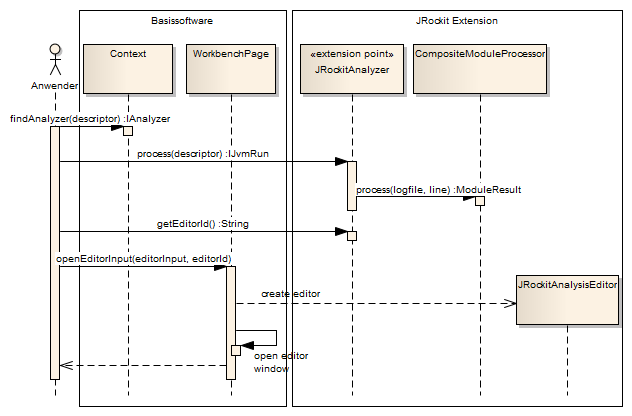
\includegraphics[width=16cm]{images/core_sequence_analysis}
	\caption{Sequenz-Diagramm Öffnen der Analyse}
\end{figure}
Der Ablauf der Garbage Collection Analyse ist folgendermassen:
\begin{enumerate}
	\item Via Context wird die Erweiterung\footnote{Erweiterungen registrieren sich als Extensions an Extension-Points. Diese Konfiguration befindet sich im plugin.xml.} gesucht.
	\item Der Analyser der Erweiterung interpretiert den Inhalt und speichert die Daten im eigenen Domänenmodell.
	\item Der Editor wird geöffnet.
\end{enumerate}

\section{Anzeige Übersicht Garbage Collection (FRQ-08)}\label{standardreport}
Der initiale Tab der Analyseseite zeigt eine Zusammenfassung der geöffneten Garbage Collection Logdatei. Die Daten werden in den Tabellen Heap Kapazität, Garbage Collection Aktivität und Gesamtstatistik angezeigt:

\subsubsection{Heap Kapazität}
\begin{itemize}
	\item Initiale und maximale Heap Kapazität
	\item Grösse Young- und Old-Space
	\item Speicherbedarf Peak, Durchschnitt: Aus den Informationen des Speicherverbrauchs vor und nach jeder Garbage Collection wird der durchschnittliche und der maximale Bedarf berechnet.
	\item Kapazität Peak, Durchschnitt: Aus den Informationen der Kapazität vor und nach jeder Garbage Collection wird die durchschnittliche und maximale Kapazität des Heaps berechnet.

\end{itemize}
\subsubsection{Garbage Collection Aktivität (Young und Old Collections)}
\begin{itemize}
	\item Letzte Garbage Collection: Zu welchem Zeitpunkt hat die letzte Garbage Collection statt gefunden.
	\item Anzahl Garbage Collections: Wieviele Garbage Collections hat es insgesamt gegeben.
	\item  Anzahl Old Collections: Wieviele Old Collections hat es gegeben.
	\item Anzahl Young Collections: Wieviele Young Collections hat es gegeben.
	\item Total Zeit der Garbage Collection: Totale Zeit, in welcher sich die Virtual Machine in der Garbage Collection befunden hat.
	\item Durchsatz der Applikation (siehe Abschnitt \ref{gc_tuning_durchsatz})

	\item Durchschnittlicher Interval in Sekunden: Durchschnittliche Pausenzeit zwischen den einzelnen Garbage Collections
	\item Durchschnittliche Dauer in Sekunden
	\item Totale Zeit der Old Garbage Collection Zyklen
	\item Totale Zeit der Young Garbage Collection Zyklen
	\item Prozentuale Zeit der Old Garbage Collection Zyklen
	\item Prozentuale Zeit der Young Garbage Collection Zyklen
\end{itemize}	

\subsubsection{Gesamtstatistik}
\begin{itemize}
	\item Dauer der Messung in Sekunden
\end{itemize}

\section{Anzeige Heap Benutzung (FRQ-09)}
Die Heap-Analyse zeigt den Verlauf des benutzten \textbf{Speichers} im Heap über die Zeit auf. Die einzelnen Garbage Collection Zyklen (Young, Old) werden verschiedenfarbig dargestellt.

\subsection{Datenquellen}
Dieser Abschnitt zeigt auf, wie die Daten für das Chart zur Anzeige der Heap Benutzung aus dem Domänenmodell geladen werden.
  \begin{longtable}{|p{1.5cm}|p{5.5cm}|p{4cm}|}
\hline
  \textbf{Achse} & \textbf{Beschreibung} & \textbf{Datenquelle\footnote{Zeigt den Pfad auf, wie auf die Daten zugegriffen wird. Siehe Abschnitt \ref{jrockit_domain_model}}}\\\hline
  X-Achse & Auf der X-Achse wird die Zeit für jeden Zustand (\textit{State}) angezeigt. & State.getTimestamp()\\\hline
  Y-Achse&Auf der Y-Achse wird der Verbrauch an Arbeitsspeicher angegeben. & State.getMemoryUsed()\\\hline
\end{longtable}

\section{Anzeige Dauer Garbage Collection (FRQ-10)}
Die \textbf{Dauer} der einzelnen Garbage Collection Zyklen wird über die Zeit aufgezeigt. Die einzelnen Garbage Collection Zyklen (Young, Old) werden verschiedenfarbig dargestellt.

\subsection{Datenquellen}
Dieser Abschnitt zeigt auf, wie die Daten für das Chart zur Anzeige der Dauer einer Garbage Collection aus dem Domänenmodell geladen werden.
  \begin{longtable}{|p{1.5cm}|p{5.5cm}|p{4cm}|}
\hline
  \textbf{Achse} & \textbf{Beschreibung} & \textbf{Datenquelle}\\\hline
  X-Achse & Auf der X-Achse wird die Zeit für jeden Zustand (\textit{State}) angezeigt. & State.getTimestamp()\\\hline
  Y-Achse&Auf der Y-Achse wird der Verbrauch an Arbeitsspeicher angegeben. & State.getTransitionEnd(). getDuration()\\\hline
\end{longtable}

\section{Profil erstellen (FRQ-11)}
Die Ansicht Profile zeigt die vom Benutzer erstellten Profile\footnote{Initial befindet sich darin allerdings nur das Standard-Profil.}. Die Beschreibung eines Analysefensters (Name, Beschreibung, Charts mit Serien, etc.) wird anhand von Profilen definiert. Es gibt folgende zwei Arten:
\begin{itemize}
	\item \textbf{Unveränderliches Profil:} Das Standard-Profil ist aktuell das einzige unveränderliche Profil. Es wird durch die \textit{JRockit Extension} definiert und kann nicht konfiguriert, verändert werden.
	\item \textbf{Veränderliches Profil:} Ein veränderliches Profil wird zur Speicherung des vom Benutzer definierten Analysefensters verwendet. Alle Änderungen die der Benutzer am Analysefenster macht (Chart hinzufügen, Chart konfigurieren), werden via ein Data-Binding an das Profil propagiert. Durch das Speichern des Profils hat der Benutzer die Möglichkeit, die selbe Analyse auch zu einem späteren Zeitpunkt an der gleichen oder einer anderen Logdatei durchzuführen.
\end{itemize}

\subsection{Domänenmodell zur Persistierung der Profile}
\textit{IConfiguration} dient zur Gruppierung von Profilen. Pro Extension wird eine Konfiguration mit verschiedenen Profilen abgelegt. Innerhalb eines Profils können unterschiedliche Diagramme (\textit{IChart}) angelegt werden, welche wiederum durch Achsen (\textit{IAxis}) und deren Datenquellen \textit{IValueProvider} definiert sind. \textit{IValueProvider} definieren den Weg, wie die Daten aus dem Domänenmodell ins Chart gelesen werden.
 \begin{figure}[H]
  	\centering
    	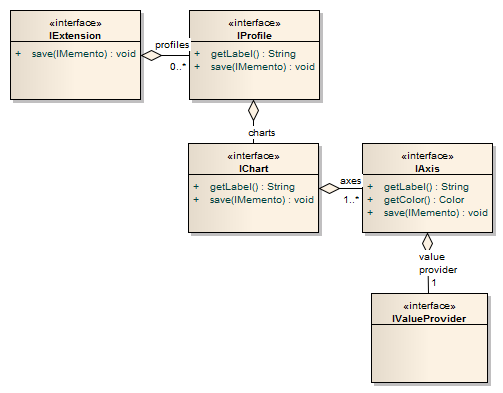
\includegraphics[width=11cm]{images/core_domain_profiles}
        	\caption{Domänenmodell: Profile}
\end{figure}

\section{Charts definieren (FRQ-12)}
Bei der Benutzung eines veränderlichen Profils hat der Benutzer die Möglichkeit, dem Analysefenster weitere Charts respektive Diagramme hinzuzufügen oder aber bereits existierende Diagramme zu manipulieren (weitere Serien hinzufügen, Serien entfernen, etc.). Die Manipulationen des Benutzers finden auf den Chart-Objekten statt und werden durch das Data-Binding propagiert. Die Administrationsoberfläche für einen Chart umfasst initial zwei Abschnitte:
\begin{itemize}
	\item Serie erstellen, definieren und hinzufügen
	 \item Serie löschen
\end{itemize}

\section{Profil speichern (FRQ-13)}
Mittels des Memento-(siehe Anhang \ref{memento}) und Visitor-Patterns\cite[S. 331]{gamma1995design} werden die Profile gespeichert.

\section{Profil exportieren, importieren (FRQ-14/ FRQ-15)}
Die Analysesoftware stellt zum Sichern und Verteilen von Profilen einen Import-Export-Mechanismus bereit. Beide sind in den Eclipse Standard-Wizards ersichtlich oder können via rechtem Mouseklick (Ansicht Profile) gestartet werden. Der Profile-Export und -Import basiert wie das Speichern auf dem im Abschnitt \ref{memento} beschriebenen Memento-Mechanismus. Zur Serialisierung in eine Datei wird das XMLMemento verwendet. 

\chapter{Konzept Qualitätsanforderungen}
\section{Hilfesystem (FRQ-16)}
Das Hilfesystem der Eclipse Entwicklungsumgebung ist als Client-Server-Lösung implementiert. Beim Start der Entwicklungsumgebung wird zusätzlich ein Jetty-Server gestartet, der die Hilfedienste wie Suche und Indexierung bereitstellt. Hilfeseiten sind auf unterschiedliche Weise verfügbar:
\begin{itemize}
\item \textbf{Indexbasierte Hilfen:} Für die generellen Informationen und Hilfen werden verschiedene Hilfeseiten basierend auf einem Index bereitgestellt. Die Inhalte sind nicht an ein Fenster oder eine Aktion des Benutzers gebunden. 
\item \textbf{Kontextsensitive Hilfen:} Tipps die im Zusammenhang mit einer Aktion oder eines Fensters stehen werden mit den kontextsensitiven Hilfen implementiert.
\end{itemize}

%--------------------------------------------
\section{Testabdeckung (QRQ-S-02)}\label{testing}
Bei Plugin-Projekten wird der Test-Code normalerweise in eigenen Fragment-Projekten abgelegt. Diese Test-Projekte werden allerdings nicht mit dem Feature ausgeliefert, sondern nur während dem Testen verwendet. Der Zugriff auf den Code der Implementation wird gewährleistet, indem aus dem Test-Projekt ein Fragment\footnote{Fragmente haben vollen Zugriff auf ihre Host-Bundles.} gemacht wird. Als Testing-Framework wird der defakto Standard JUnit verwendet. JUnit ist sowohl von allen Entwicklungsumgebungen als auch von Maven und Tycho unterstützt.

\section{Internationalisierung (QRQ-S-03))}
Die Analysesoftware kann in den Sprachen Deutsch und Englisch gestartet werden. Die gewählte Sprache wird von der Entwicklungsumgebung übernommen\footnote{Die Entwicklungsumgebung übernimmt die Sprache der Java Lauzeitumgebung: Voreinstellung oder Auswahl über Kommandozeile (-nl de). } und kann nicht via ein Menu geändert werden. 
Basierend auf der \textit{Locale}-Klasse der Java Laufzeitumgebung können sprachabhängige Ressourcen geladen werden. Sprachabhängig sind folgende Bereiche:
\begin{itemize}
	\item \textbf{Texte, Labels im Code:} Eclipse stellt zur Externalisierung von Strings einen Wizard zur Verfügung. Die Texte werden in Properties-Dateien extrahiert und beim Starten der Applikation geladen.
	\item \textbf{Texte, Labels in Deskriptoren:} Die sich in den Eclipse-Deskriptoren (plugin.xml und Manifest.MF) befindenden sprachabhängigen Texte wie Organisation, Plugin-Name und -Beschreibung werden ebenfalls in Properties-Dateien extrahiert. Der Ort und Name dieser Dateien ist per Konvention \textit{\textbackslash \$\{plugin\}\textbackslash OSGI-INF\textbackslash I10n\textbackslash bundle\_\$\{lang\}.properties}. Der Inhalt wird vom Eclipse-Framework geladen.
	\item \textbf{Hilfesystem:} Eclipse startet zur Anzeige des auf HTML basierenden Hilfesystems einen Webserver. Die Hilfeseiten können ebenfalls in unterschiedlichen Sprachen definiert werden und werden auf der Basis der gewählten Locale angezeigt.
\end{itemize} 

\section{Usability (QRQ-S-04))}
Einige der Funktionalitäten der Analysesoftware wie Beispielsweise das Einlesen und Parsen der Logdateien dauern lange. Der Benutzer benötigt eine Statusinformation. Operationen dieser Art werden mittels des Eclipse \textit{IProgressService} gestartet. Dies hat für die Applikation und den Benutzer folgende Vorteile:
\begin{itemize}
	\item \textbf{Nebenläufigkeit:} Die Applikation startet die Arbeit in einem eigenen nicht-UI Thread\footnote{Einem Thread der nicht für das Zeichnen des Benutzerinterfaces verwendet wird.}, sodass es nicht zu Nebeneffekten wie einem eingefrorenen Bildschirm kommt. Der Benutzer kann die Fortschrittsanzeige minimieren und mit der Applikation weiterarbeiten.
	\item \textbf{Fortschrittsanzeige: } Die Applikation teilt dem Benutzer über eine Anzeige mit, bei welcher Position sich der Prozess befindet und wie viel Arbeit prozentual bereits gemacht wurde.
	\item \textbf{Unterbrechbarkeit: } Der Prozess erkundigt sich periodisch bei der Monitoring-Komponente ob er durch den Benutzer abgebrochen wurde. Sobald dies der Fall wäre, würde er die Arbeit beenden und das bereits Erledigte aufräumen.
\end{itemize}


\section{Korrektheit (QRQ-S-05))}
Um mit Java-Applikationen genaue Werte zu berechnen wird von \cite{bloch2008effective} empfohlen, die Klasse \textit{BigDecimal} anstelle von \textit{Double} und \textit{Long} zu verwenden. Die in der Analysesoftware verwendeten Werte werden mit einer Genauigkeit von 0.1 gerechnet.

\chapter{Infrastruktur}\label{konzept_3}
Build-Automatisierung, Issue Tracking und Versionsverwaltung sind im Context der Analysesoftware. Dieser Abschnitt beschreibt die eher administrativen Belange und definiert das Projektsetup. 

\section{Verwendete Werkzeuge}
\subsection{Build-Automatisierung}
Die Automatisierung des Software-Builds ist hinsichtlich der Integration in ein Continuous Integration System wichtig. Zusätzlich entfallen so zeitaufwändige Tasks wie die Paketierung und das Deployment der Applikation.
Als Werkzeug zum automatisierten Build der Software wird Maven Tycho\footnote{Im Bereich der Eclipse Rich Client Entwicklung kann entweder PDE Build, ein auf Apache Ant basiertes Build-System für Eclipse RCP Applikationen\cite{vogelZapfPdeBuild} oder die Maven-Integration Tycho (http://tycho.sonatype.org) verwendet werden.} verwendet.

Tycho ist relativ neu und bringt im Vergleich mit dem PDE Build einige Vorteile mit sich:
\begin{itemize}
	\item Maven folgt dem Prinzip ``Convention over Configuration''\footnote{Das Prinzip ``Convention over Configuration'' hat zur Folge, dass im Wesentlichen nur von den Standardeinstellungen abweichende Werte konfiguriert werden müssen.} - die Konfiguration des Builds wird dadurch wesentlich einfacher.
	\item Maven ist de facto Standard bei den Build-Werkzeugen.
\end{itemize}

\subsection{Issue Tracker}\label{issue_tracker}
Als Issue Tracker wird Jira verwendet. Es handelt sich dabei um eine kostenpflichtige aber relativ günstige Software für die Verwaltung von Bugs, Feature-Requests, etc. Sie lässt sich auch gut mit allen gängigen Systemen zur Versionsverwaltung integrieren.

\subsection{Versionsverwaltung}
Als Versionsverwaltungssysteme kommen mehrere Werkzeuge in Frage, darunter befinden sich auch CVS und Subversion. Git\footnote{http://git-scm.com} ist ein verteiltes Versionsverwaltungssystem und ist konzeptionell und hinsichtlich Benutzerfreundlichkeit besser als Subversion und CVS\footnote{Git kann offline verwendet werden, das Verschieben von Verzeichnissen führt nicht zu Problemen, etc.}. Die Charakteristik des Systems erfordert es nicht unbedingt, dass es ein zentrales Repository gibt. Ein Repository befindet sich auf jedem Client. Trotzdem setzt man in der Regel ein zentrales Repository auf, in welches die Entwickler jederzeit commiten können. Eine empfehlenswerte Einführung in Git kann unter \cite{dilger201111}  gefunden werden.

Auf der Plattform Github\footnote{http://github.com} kann man Git-Projekte frei ``hosten''.




\subsection{Continous Integration}
Continuous Integration Systeme dienen zur Steigerung der Softwarequalität. Sie machen dies in der Regel, indem sie alle Tests und den Gesamtbuild der Software periodisch - beispielsweise jede Stunde - durchführen. Für dieses Projekt sind einige Voraussetzungen gegeben:
\begin{itemize}
	\item \textbf{Buildwerkzeug Maven:} Das System muss Maven als Build- und Automatisierungswerkzeug unterstützen.
	\item \textbf{Git Versionskontrolle:} Der Quelltext der Applikation muss via Git vom Sourcecode Repository ausgecheckt werden können.
	\item \textbf{Freie Lizenz:} Die Software muss mindestens frei verfügbar sein oder open-source.
\end{itemize}
In den letzten Jahren hat sich Hudson\footnote{Vor kurzem haben sich einige Entwickler von Hudson aufgrund von Streitigkeiten mit Oracle dazu entschieden, die Software weiter unter dem Namen Jenkins zu entwickeln.} in vielen Projekten durchgesetzt. Hudson ist eine open-source Continuous Integration Software die gegenüber anderen Systemen einige Vorteile mit sich bringt:
\begin{itemize}
\item Hudson ist open-source.
\item Hudson ist sehr einfach zu installieren und administrieren.
\item Hudson basiert auf einem Plugin-System und ist aufgrund dessen erweiterbar. Es gibt Plugins für die Integration von Maven-Projekten und den Zugriff auf Git Repositories.
\end{itemize}

\section{Konfigurationsmanagement}
Jedes Deployment entspricht einer Version in Jira (siehe Abschnitt \ref{issue_tracker}).
Ab dem ersten Release entspricht die Versionsnummer folgendem Muster:
\begin{center}
\fbox{\textbf{\textless Major\textgreater.\textless Minor\textgreater .\textless Build\textgreater}}
\end{center}

\textbf{Ein Beispiel für eine Versionsnummer wäre 1.3.1. Gestartet wird mit 1.0.0}. 
\subsection{Pflege der einzelnen Versionen}
\begin{itemize}
\item \textbf{Build:} Bei jedem Bugfix- und/oder sonstigen ausserordentlichen Zwischenrelease, wird die Build-Version um eins hochgezählt.
\item \textbf{Minor:} Bei jedem Feature-Deployment während einem ordentlichen Release, wird die Minor-Version um eins hochgezählt.
\item \textbf{Major:} Bei grossen Änderungen und/oder Entwicklungen von Zusatzmodulen wird die Major-Version um eins hochgezählt.

\end{itemize}


\subsection{Versionsverwaltung}
Das zentrale Repository dieses Projektes befindet sich auf Github\footnote{https://github.com/schmidic/bachelorthesis}. Es ist jederzeit verfügbar und kann von allen Clients (Entwickler, Continuous Integration) jederzeit angesprochen werden. Ein neuer Entwickler klont das Repository auf seinen Rechner, um am Sourcecode arbeiten zu können.
\subsubsection{Übersicht}
Das Repository besteht aus drei Branches:
\begin{itemize}
\item \textbf{master:} Auf dem \textit{master}-Branch befindet sich der aktuelle Entwicklungsstand. 
\item \textbf{release:} Nur vom \textit{release}-Branch wird in die Produktion deployt. Dadurch kann jederzeit am produktiven System ein Bugfix gemacht werden. Der \textit{release}-Branch entspricht der aktuell deployten produktiven Applikation.
\item \textbf{next:} Auf dem \textit{next}-Branch werden zukünftige Features entwickelt, die noch nicht in die Produktion deployt werden sollen.
\end{itemize}

\subsubsection{Bugfix Entwicklung}
Ein Bugfix der produktiven Applikation findet auf der Basis des \textit{release}-Branches statt. Dazu wird daraus allerdings ein neuer Branch erzeugt. Die Minor-Version für den Bugfix wird um eins inkrementiert. Ausgehend von einem Beispiel zweier Bugfixes für die Version 1.0.0 ist der Ablauf wie folgt:
\begin{enumerate}
\item Für den laufenden Release (Version 1.0.0) werden die Bugs (\#4321, \#4322) im Jira rapportiert.
\item Der Entwickler checkt den \textit{release}-Branche aus und erstellt daraus einen neuen Branch (\textit{bugfix-for-1.0.0}).
\item Der Entwickler inkrementiert die Maven-Version um eins (neu 1.0.1).
\item Der Entwickler erstellt eine neue Jira Version (1.0.1).
\item Der Entwickler repariert die Fehler, die Applikation wird getestet.
\item Die Bugs innerhalb des Jiras werden der neuen Version zugeordnet.
\item Der Entwickler führt (merge) die Bugfixes zurück in den \textit{release}-Branch. Die Zuordnung der Commits mit den Jira-Bugs wird über den Kommentar in der Versionsverwaltung mit dem Bug im Jira verlinkt. Die Anpassung des Kommentars der vorherigen Commits kann mittels einem Rebasing (siehe \cite{dilger201111}) gemacht werden.
\item Erstellen eines Tags für den Release
\item Release der neuen Version (1.0.1).
\end{enumerate}
Mit dem dedizierten \textit{release}-Branch kommt ein wesentlicher Vorteil zum Tragen: Man kann ein Bugfix Release in das Produktivsystem veranlassen, der nur einen bestimmten Bugfix enthält, selbst wenn auf dem \textit{master} eventuell schon weitere Features entwickelt wurden.

\subsubsection{Feature Entwicklung}
Die Entwicklung eines Features, welches in die Produktion einfliessen soll, wird auf dem Master-Branch durchgeführt. Um Konflikte mit dem \textit{release}-Branch zu vermeiden, wird nach jedem Release zumindest die Minor-Version des \textit{master}-Branches um eins erhöht.  Das Vorgehen ist wie folgt:
\begin{enumerate}
\item Für den laufenden Release gibt es die Feature-Requests (\#4351, \#4352) im Jira.
\item Der Entwickler checkt den \textit{master}-Branch (Version 1.0.0) aus und erstellt daraus einen neuen Branch (\textit{feature-1.1.0})
\item Der Entwickler inkrementiert die Maven-Version (1.1.0).
\item Der Entwickler erstellt eine neue Jira Version (1.1.0).
\item Der Entwickler erstellt das neue Feature.
\item Der Entwickler ordnet die Feature-Requests im Jira der neu erstellten Version zu.
\item Der Entwickler führt (merge) den \textit{feature-1.1.0}-Branch zurück in den \textit{master}-Branch.  Die Zuordnung der Commits mit den Jira-Bugs wird über den Kommentar mit dem Jira-Bug verlinkt. Die Anpassung des Kommentars der vorherigen Commits kann mittels einem Rebasing (siehe \cite{dilger201111}) gemacht werden.
\end{enumerate}
\part{Umsetzung}
\chapter{Implementation}\label{implementation}
Im Proof of Concept wurden die Anforderungen folgendermassen umgesetzt.\footnote{Kann auch im Abschnitt \titleref{bedienungsanleitung} oder an der laufenden Software überprüft werden.}:
\section{Funktionale Anforderungen}
Die funktionalen Anforderungen konnten alle umgesetzt werden. Dieser Abschnitt beschreibt etwas detaillierter, was wie umgesetzt werden konnte.

\subsection{Installation (FRQ-01) und Update (FRQ-02)}
Installation und Update der beiden Features Core und JRockit Extension können über die Update-Seite gemacht werden. Beide Funktionalitäten sind Bestandteil des Eclipse-Frameworks und werden via ein Update-Site-Plugin und die beiden Feature-Plugins bereitgestellt.

\subsection{Datei importieren (FRQ-03)}
Die Dateien werden in eine eigens dafür registrierte View importiert. Das Speichern und Wiederherstellen des Zustands dieser View findet über das von Eclipse implementierte Memento-Pattern (siehe Anhang \ref{memento}) statt. 

\subsection{Datei einlesen (FRQ-04)}
Die eingelesene Datei wird in Form des im Konzept beschriebenen Domänenmodells ins Memory geladen. 

\subsection{Garbage Collection Logdatei parsen (FRQ-05)}
Die Log-Ausgaben des Memory-Moduls (Debug-Level: info) werden mittels Regulären Ausdrücken geparst und in strukturierter Form gespeichert. Strukturiert meint eine objektorientierte Form der Daten (siehe Abschnitt \ref{jrockit_domain_model}).

\subsection{Standardauswertung anzeigen (FRQ-06)}
Für die importierten Dateien besteht die Möglichkeit, sie in der Standardauswertung darzustellen. Die Standardauswertung zeigt die im Konzept definierten Ansichten, Tabs (siehe Abschnitt \titleref{standardreport} auf Seite \pageref{standardreport}).

\subsection{Profil erstellen (FRQ-07)}
Profile können durch den Benutzer erstellt und an seine Bedürfnisse angepasst werden. Das Anpassen beinhaltet die Definition von eigenen Charts und deren Datenserien. Das Speichern, Exportieren und Importieren wird über das von Eclipse implementierte Memento-Pattern (siehe Anhang \ref{memento}) gemacht.

\subsection{Hilfesystem (FRQ-08)}
Das Hilfesystem wurde sowohl für die contextsensitive wie auch die indexbasierte Hilfe angelegt. Aktuell sind alle existierenden Hilfeseiten in den Sprachen Deutsch und Englisch vorhanden, diese können aber ohne Entwicklungsaufwand auch um weitere Sprachen ergänzt werden. 

\section{Qualitätsanforderungen Software}
\subsection{Erweiterbarkeit (QRQ-S-01)}
Die Analyse der JRockit Dateien wurde als Erweiterung implementiert. Es besteht die Möglichkeit, dass sich Erweiterungen für andere Log-Dateien bei der Basissoftware registrieren, die dann das Parsen und Aufbereiten der Datei durchführt und die Analysen durchführt.

\subsection{Testabdeckung (QRQ-S-02)}
Die Testabdeckung entspricht nicht den Anforderungen von 80 Prozent. 

\subsection{Internationalisierung (QRQ-S-03)}
Viele der eingebauten Namen und Labels sind bereits zweisprachig (Englisch, Deutsch) definiert. Die restlichen müssen noch übersetzt und in die Sprachressourcen extrahiert werden.

\subsection{Usability (QRQ-S-04)}
Lange dauernde Operationen (Einlesen, Parsen der Daten) werden vom Eclipse-Framework asynchron gestartet. Dem Benutzer wird ein Progress-Monitor angezeigt, in welchem er die Operation auch abbrechen kann.

\subsection{Korrektheit (angezeigte Werte) (QRQ-S-05)}
Um mit Java-Applikationen genaue Werte zu berechnen wird von \cite{bloch2008effective} empfohlen, die Klasse \textit{BigDecimal} anstelle von \textit{Double} und \textit{Long} zu verwenden. Die in der Analysesoftware verwendeten Werte werden mit einer Genauigkeit von 0.1 gerechnet.

\chapter{Review und Ausblick}
\section{Was leistet das Tool?}

\section{Was leistet das Tool (noch) nicht?}







\chapter{Glossar}\label{glossar}
  \begin{longtable}{|p{4.5cm}|p{6cm}|p{4.1cm}|}
\hline
  \textbf{Wort} & \textbf{Beschreibung} & \textbf{Herkunft}\\\hline
  Continuous Integration  & Kontinuierliches Kompilieren, Bilden und Testen einer Applikation. Hilft einem oder mehreren Entwicklern eine bessere Softwarequalität zu erreichen.&-\\\hline
  Bundle (Eclipse) & siehe Plugin & siehe Plugin\\\hline
  Category (Eclipse) & Auf einer Eclipse Update-Seite werden Features zur Verfügung gestellt. Diese können logisch noch einmal in Kategorien unterteilt werden. & Eclipse\\\hline
  Feature (Eclipse) & Als Feature verpackt man im Eclipse-Umfeld eine logische Einheit an Funktionalität. & Eclipse\\\hline
  Fragment & Manchmal macht es im Eclipse-Umfeld Sinn, gewisse Teile der Applikation optional zu definieren. In diesem Fall verwendet man Fragmente. Sie erlauben die Erweiterung eines bestehenden Bundles (\textit{Host-Bundle}) und haben Zugriff auf alle auch nicht exportierten Packete dieses Host-Bundles. Test-Projekte werden oft auch als Fragmente definiert, da ihnen der volle Zugriff auf das \textit{Host-Bundle} gewährleistet wird. & Eclipse\\\hline
  Data Binding & Data Binding ist ein Mechanismus in Desktop Applikationen, um die Werte eines Bedienelementes mit dem hinterlegten View-Model zu verbinden. Änderungen am Wert des Eingabefeldes werden beispielsweise an das Model propagiert. Sofern es sich um ein bidirektionales Binding handelt, auch umgekehrt.  & - \\\hline
  Old Collection & Eine Old Collection bezeichnet die Garbage Collection auf der Old Generation. & Speichermanagement\\\hline
  Old Generation & Bei einigen Garbage Collection Algorithmen wird der Heap in Generationen unterteilt. Der Bereich mit den jungen Objekten wird Old Generation genannt.  & Speichermanagement \\\hline
  Parseprozess & Bezeichnet die Interpretation und Aufbereitung von unstrukturierten Daten in eine strukturierte Form (Domänenmodell, Liste, Key-Value Datenstruktur, etc.). & Compilerbau \\\hline
  Plugin (Eclipse) & Ein Plugin ist eine technische Trennung von gewissen logischen Softwareteilen. Dabei definiert man die Schnittstelle zu anderen Plugins mittels einer Manifest.mf respektive einer plugin.xml Datei. Diese definieren die Abhängigkeiten, die Exportierten Klassen und die Erweiterungspunkte.  & Eclipse\\\hline
Rich Client Framework & Software-Bibliothek, mittels welchem sich Rich Client Applikationen entwickeln lassen. & -\\\hline
Rich Client Plattform & Der Begriff Rich Client Plattform wird in diesem Dokument oft als Synonym für Desktop- respektive Client-Applikation verwendet. & Vor gut 10 Jahren verlagerte sich die Logik vom Client auf den Server. Jede Interaktion mit dem System fand über eine Verbindung zum Server statt, der Client stellte die Inhalte nur dar. Die Anwendungen waren wenig benutzerfreundlich. Es gab deshalb eine Gegenbewegung zu den Rich Client Applikationen, dabei wird mindestens ein Teil der Logik wieder in den Client verlagert.\\\hline
  Update Site & Eine Update-Seite im Eclipse-Umfeld ist eine per Konvention aufgebaute Webseite die via das Http-Protokoll zugänglich ist und Software-Komponenten (Features) enthält.& Eclipse\\\hline
  Virtual Machine (JRockit, HotSpot) & Laufzeitumgebung die beispielsweise eine Java Applikation ausführt. & Softwareentwicklung  \\\hline
  Wizard & Dialog innerhalb einer Anwendung, der den Benutzer durch einen Prozess führt. & -\\\hline
  Young Collection & Eine Young Collection bezeichnet die Garbage Collection auf der Young Generation.  & Speichermanagement\\\hline
  Young Generation &  Bei einigen Garbage Collection Algorithmen wird der Heap in Generationen unterteilt. Der Bereich mit den jungen Objekten wird Young Generation genannt.  & Speichermanagement \\\hline
User Interface &  Als User Interface (Benutzeroberfläche) werden alle Schnittstellen zwischen Mensch und Maschine bezeichnet. Diese können textbasiert oder grafisch sein (GUI). &  -\\\hline
      \caption{Glossar}\\
  \end{longtable}



\chapter*{Abkürzungen}\label{abkuerzungen}
\addcontentsline{toc}{chapter}{Abkürzungen}
  \begin{longtable}{|p{3cm}|p{5cm}|p{6cm}|}
      \caption{Glossar}\\
\hline
  \textbf{Abkürzung} &\textbf{Begriff} &  \textbf{Beschreibung} \\\hline
  GC & Garbage Collection & \\\hline
Unit under Test & Unit under Test & Von Unit under Test spricht man bei der zu testenden Klasse.\\\hline
  \end{longtable}



\bibliography{bachelorthesis_rschmid}
\lstlistoflistings
\addcontentsline{toc}{chapter}{Listings}
\listoffigures
\addcontentsline{toc}{chapter}{Abbildungsverzeichnis}
\listoftables
\addcontentsline{toc}{chapter}{Tabellenverzeichnis}
\part*{Anhang}
\appendix
\chapter{Eclipse Rich Client Framework}
\section*{Zustand von Komponenten speichern}\label{memento}
Die Speicherung des Zustands einer View wird von Eclipse unterstützt, indem die Methode \textit{saveState(memento:IMemento)} von \textit{ViewPart} implementiert wird. \textit{IMemento} ist eine Eclipse-Klasse und gleichzeitig die Abstraktion eines Mementos. Memento ist ein Design Pattern und wurde durch die Gang of Four\footnote{Erich Gamma, Richard Helm, Ralph Johnson, John Vlissides} in \cite[S. 283]{gamma1995design} zum ersten Mal definiert. Mementos dienen zur Serialisierung von Objekten und eignen sich besonders zur Persistierung von hierarchischen Strukturen. Das Eclipse-Framework speichert die Zustände von Views mittels eines XMLMemento im Eclipse-Context ab. Die Initialisierung der Komponente wird wiederum durch das Überschreiben der Methode \textit{init(site:IViewSite, memento:IMemento)} der Klasse \textit{ViewPart} gemacht.

\chapter{Bedienungsanleitung}\label{bedienungsanleitung}
\section*{Installation der Software}
Eclipse Installationsdialog mit Menu \textit{Hilfe / Neue Software installieren} öffnen.
 \begin{figure}[H]
  	\centering
    	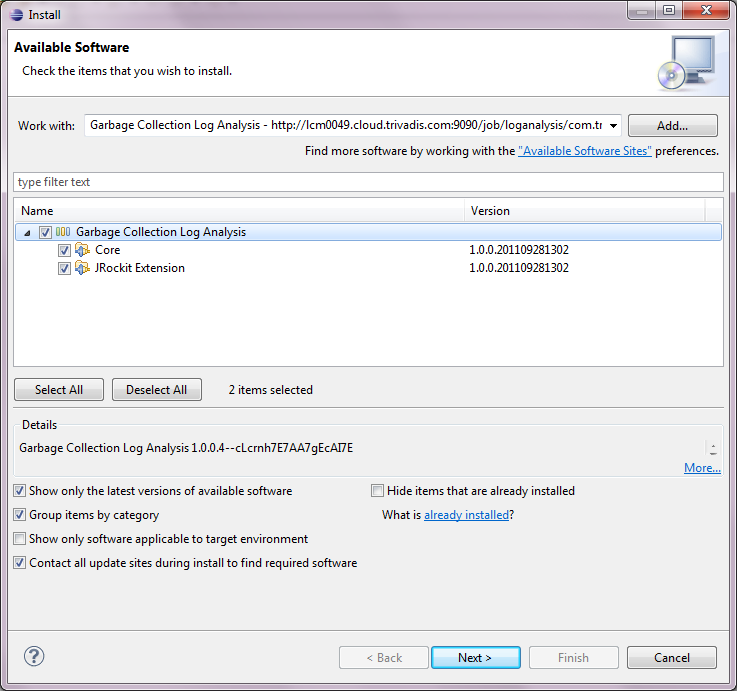
\includegraphics[width=10cm]{images/tutorial_install01}
        	\caption{Installation Garbage Collection Log Analyse}
\end{figure}
Durch Angabe der Update-Seite können danach beide Features ausgewählt werden. Nach zweimaligem Klick auf \textit{Weiter} und anschliessender Bestätigung der Lizenzbestimmungen wird die Software installiert. Danach muss die Entwicklungsumgebung neu gestartet werden.


\section*{Update}
Wenn ein Update der Software verfügbar ist, kann via \textit{Hilfe / Nach Updates suchen} das Update-Fenster geöffnet werden. Die  Softwarepakete werden heruntergeladen und aktualisiert.
 \begin{figure}[H]
  	\centering
    	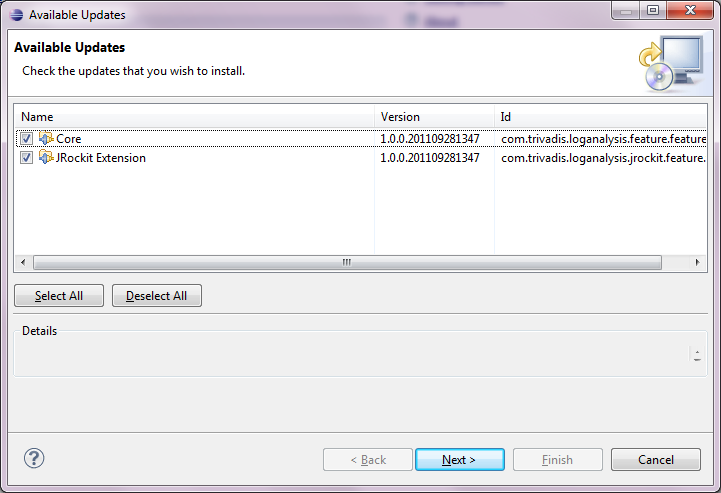
\includegraphics[width=10cm]{images/tutorial_update01}
        	\caption{Update Garbage Collection Log Analyse}
\end{figure}

\section*{Dashboard}
Nach der Installation kann über den Knopf \textit{GC Log Analyse Dashboard} in der Toolbar das Dashboard geöffnet werden. 
 \begin{figure}[H]
  	\centering
    	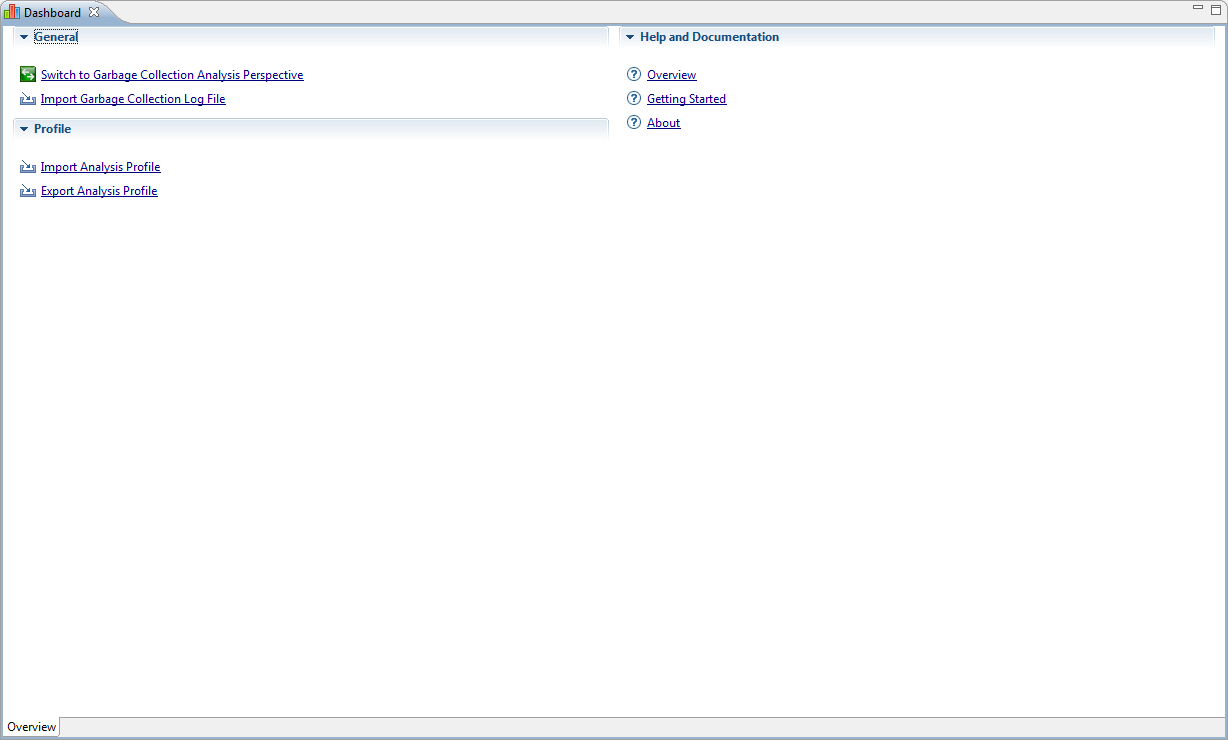
\includegraphics[width=16cm]{images/tutorial_dashboard}
        	\caption{Dashboard}
\end{figure}

Auf dem Dashboard befinden sich verschiedene Abschnitte mit unterschiedlichen Funktionen:
\begin{itemize}
	\item Generell 
		\begin{itemize}
			\item Wechsel in die Garbage Collection Perspektive
			\item Import einer Garbage Collection Logdatei
		\end{itemize}
	\item Profile
		\begin{itemize}
			\item Import eines Analyseprofils
			\item Export eines Analyseprofils
		\end{itemize}
	\item Hilfe und Dokumentation
		\begin{itemize}
			\item Beinhaltet Links auf verschiedene Inhalte der Hilfe
		\end{itemize}
\end{itemize}

\section*{Import einer Garbage Collection Logdatei}
Der Import-Wizard kann auf verschiedene Arten geöffnet werden:
\begin{itemize}
	\item Über Rechtsklick auf die View \textit{Logdateien} / \textit{Import Garbage Collection Logdatei}.
	\item Über \textit{File / Import / Import Garbage Collection Logdatei} (Kategorie: Garbage Collection)
	\item Im Dashboard über \textit{Import Garbage Collection Logdatei}
\end{itemize}

Über den \textit{Browse} Button muss der Ordner angegeben werden, welcher die Logdateien beinhaltet. Anschliessend kann die Logdatei im darunterliegenden Fenster selektiert werden. Mit Klick auf \textit{Finish} wird die Datei importiert.
 \begin{figure}[H]
  	\centering
    	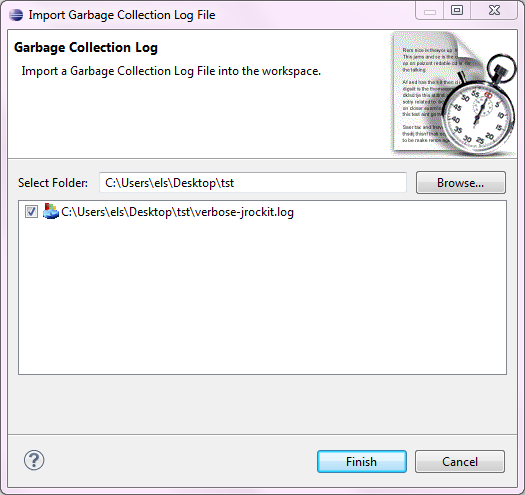
\includegraphics[width=10cm]{images/tutorial_importlog}
        	\caption{Logdatei importieren}
\end{figure}

\section*{Profile}
Zur Verwaltung der verschiedenen Analyseprofile gibt es die View \textit{Profile}. In ihr können Profile erstellt, exportiert und importiert werden. Wenn eine Logdatei mit einem bestimmten Analyseprofil geöffnet werden soll, muss das entsprechende Profil darin selektiert sein.

\subsection*{Profil erstellen}
Mit Rechtsklick auf die Ansicht \textit{Profile / Profil erstellen} oder \textit{Datei / Neu / Andere... / Analyse Profil} (Kategorie Garbage Collection) kann der Dialog zum Erstellen eines neuen Profils geöffnet werden. 
 \begin{figure}[H]
  	\centering
    	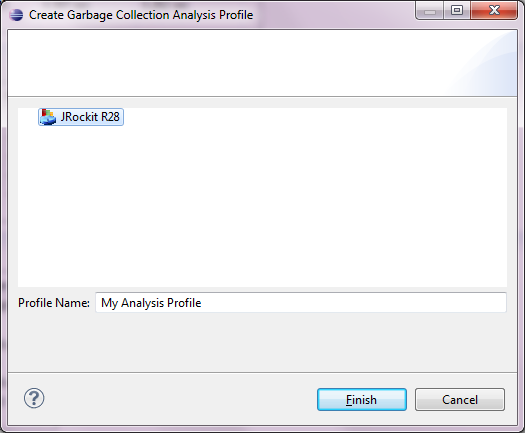
\includegraphics[width=10cm]{images/tutorial_newprofile}
        	\caption{Profil erstellen}
\end{figure}
Sofern die Erweiterung, für die das Profil erstellt wird, selektiert und ein Name vergeben ist, wird mittels Klick auf \textit{Fertigstellen} das Profil angelegt.

\subsection*{Profil exportieren}
Mit Rechtsklick auf die Ansicht \textit{Profile} und Auswahl von \textit{Profil exportieren}, können die Profile in eine Lap\footnote{Lap steht für Log Analysis Profile}-Datei exportiert werden.
 \begin{figure}[H]
  	\centering
    	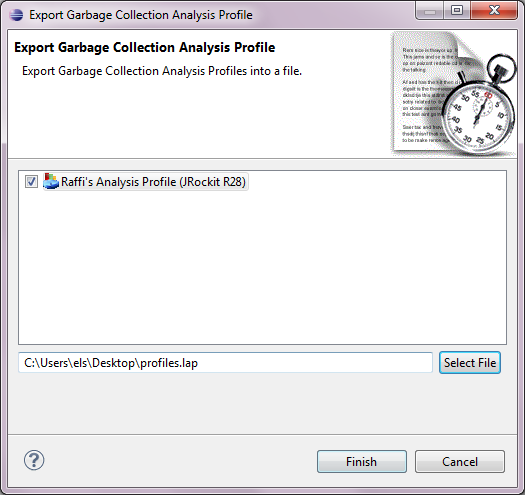
\includegraphics[width=10cm]{images/tutorial_exportprofile}
        	\caption{Profil exportieren}
\end{figure}

\subsection*{Profil importieren}

Mit Rechtsklick auf die Ansicht \textit{Profile / Profil Importieren} können die Profile aus einer Lap-Datei importiert werden.
 \begin{figure}[H]
  	\centering
    	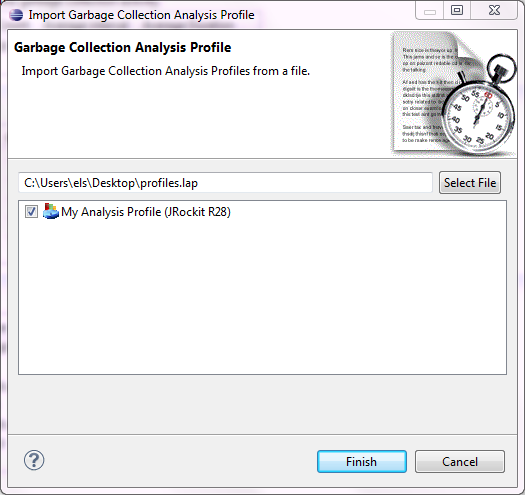
\includegraphics[width=10cm]{images/tutorial_importprofile}
        	\caption{Profil importieren}
\end{figure}

\section*{Garbage Collection Analyse}
\subsection*{Standardauswertung}
Sofern in der Ansicht \textit{Profile} kein Profil selektiert ist, wird mit Doppelklick auf eine importierte Logdatei die Standardauswertung geöffnet. Die Standardauswertung besteht aus drei unterschiedlichen Tabs. Der erste Tab zeigt eine Zusammenfassung der Garbage Collection, der zweite Tab den Verlauf des benötigten Speichers auf dem Heap über die Zeit, und der dritte Tab die Dauer der einzelnen Garbage Collection Zyklen über die Zeit. 

\subsubsection*{Zusammenfassung}
 \begin{figure}[H]
  	\centering
    	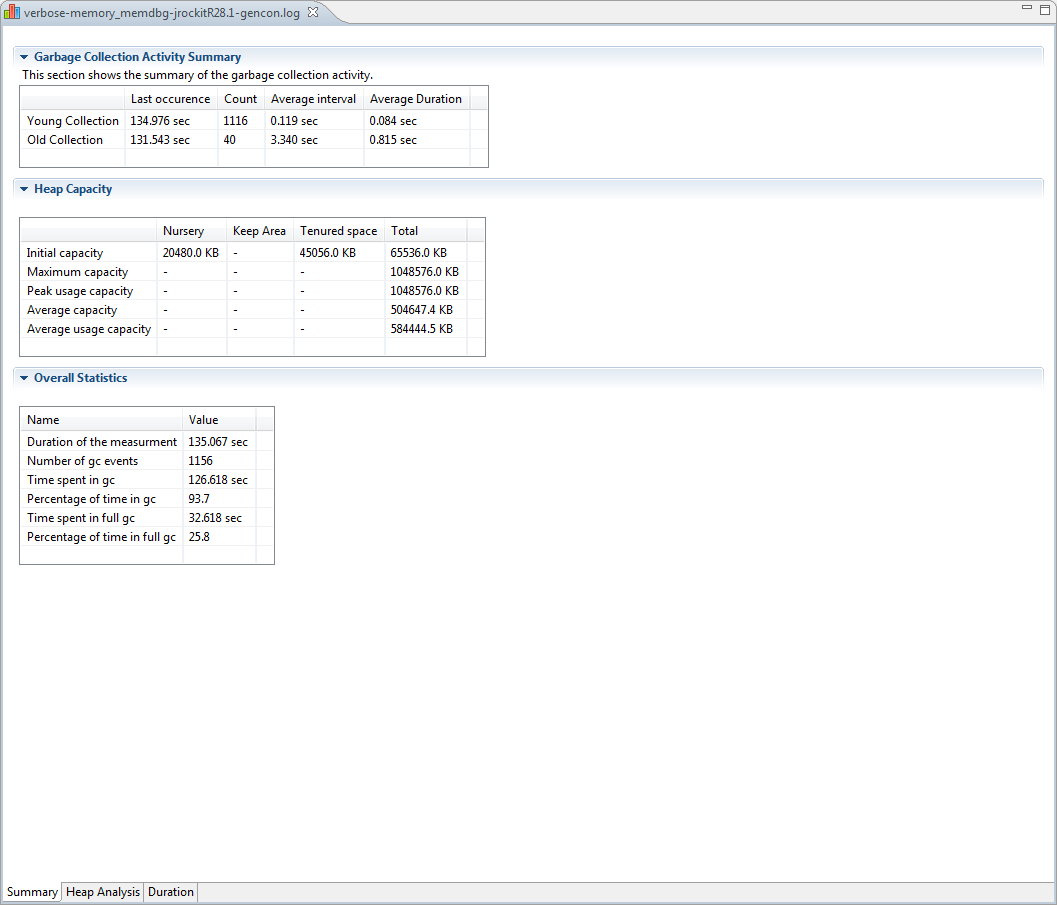
\includegraphics[width=15cm]{images/tutorial_standardreport_statistics}
        	\caption{Standardauswertung: Zusammenfassung}
\end{figure}

\subsubsection*{Heap Analyse}
 \begin{figure}[H]
  	\centering
    	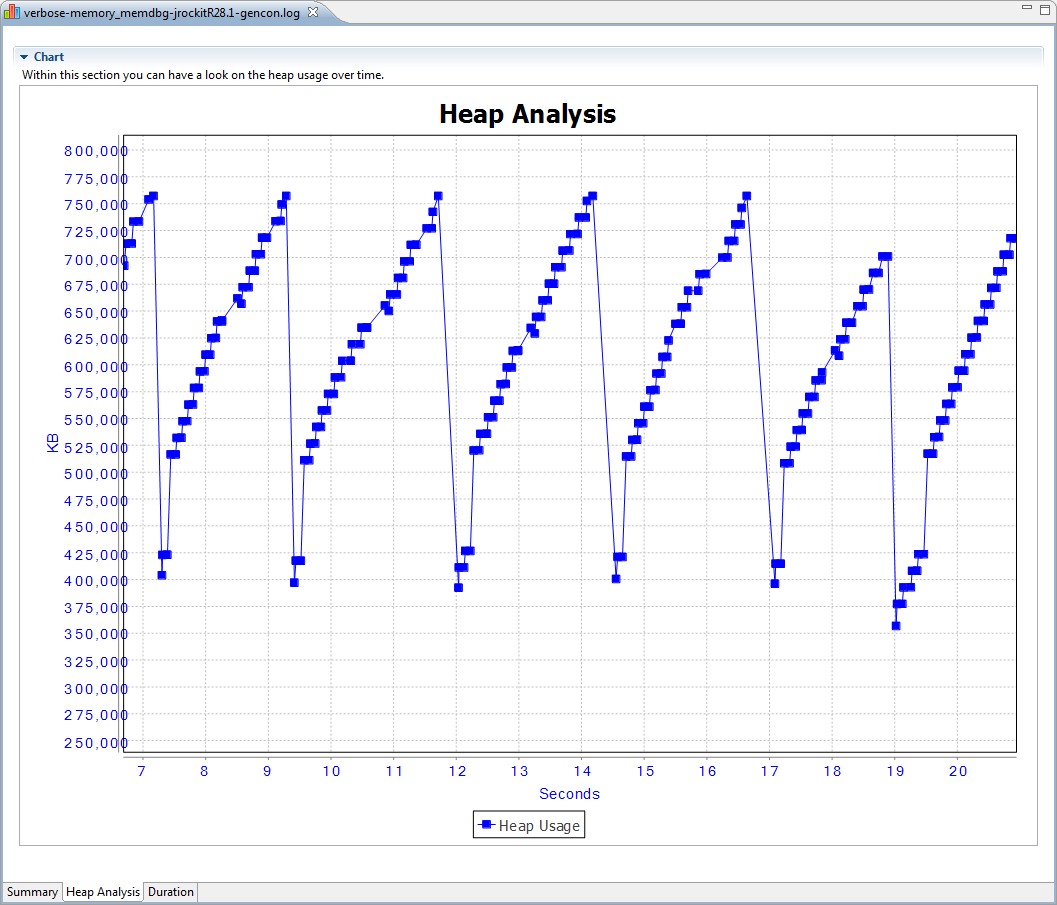
\includegraphics[width=15cm]{images/tutorial_standardreport_heapanalysis}
        	\caption{Standardauswertung: Heap Analyse}
\end{figure}

\subsubsection*{Dauer Garbage Collection}
 \begin{figure}[H]
  	\centering
    	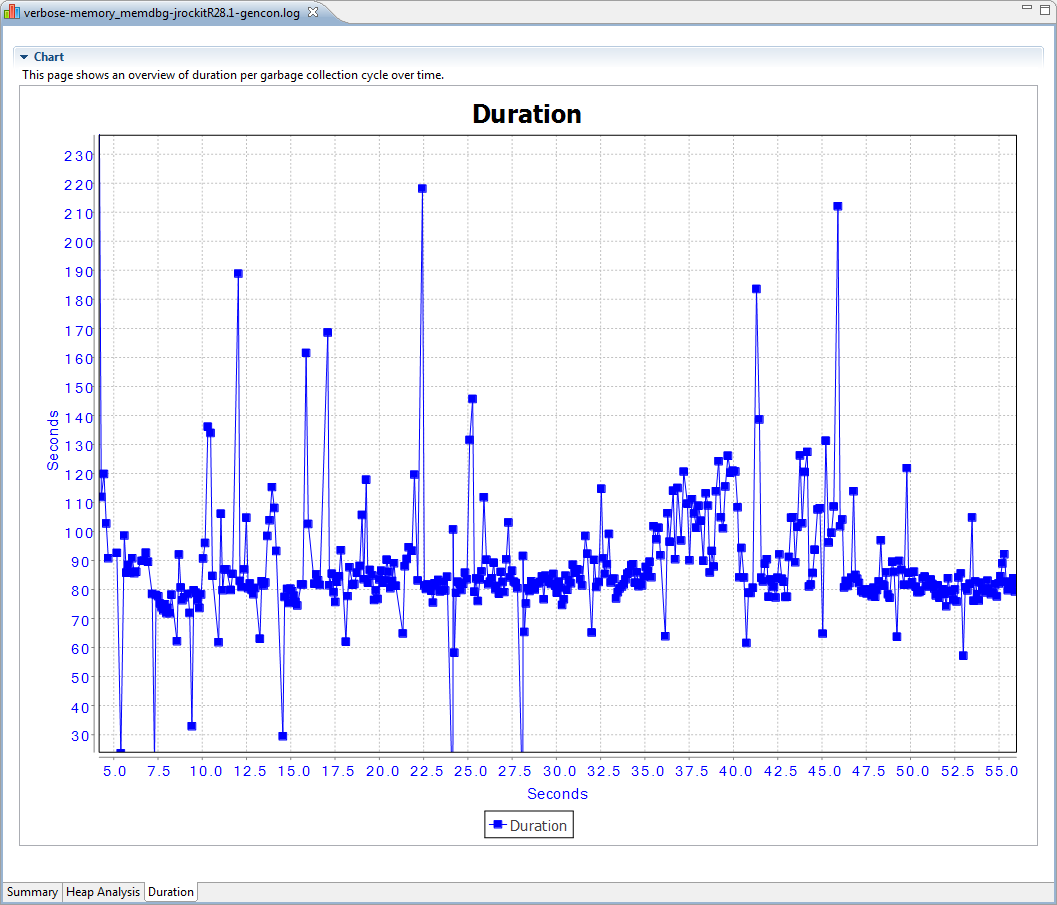
\includegraphics[width=15cm]{images/tutorial_standardreport_duration}
        	\caption{Standardauswertung: Dauer Garbage Collection}
\end{figure}



\subsection*{Benutzerdefinierte Auswertung (Profile)}
Die benutzerdefinierte Auswertung wird geöffnet, indem man vor dem Öffnen einer Datei in der Ansicht \textit{Profile} ein Profil selektiert. 
 \begin{figure}[H]
  	\centering
    	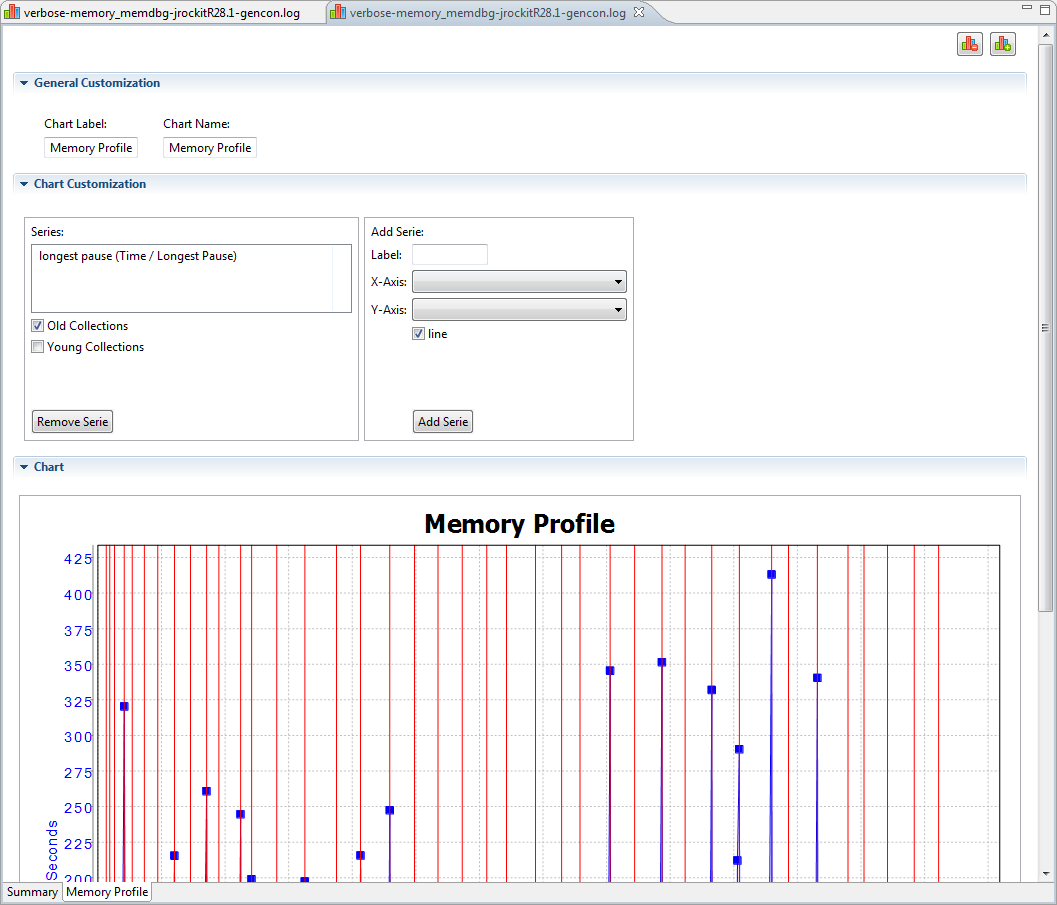
\includegraphics[width=15cm]{images/tutorial_custom_report}
        	\caption{Benutzerdefinierte Auswertung definieren}
\end{figure}
Im Abschnitt \textit{Generelle Anpassungen} können die Namen von Tab  und Diagramm definiert werden. Im Abschnitt \textit{Anpassung Diagramm} können neue Serien auf das Diagramm hinzugefügt werden. Dabei können pro Serie die Werte für X-, Y-Achse und ein paar Eigenschaften angegeben werden. Das jeweilige Ende einer Garbage Collection kann als vertikale Linien in rot (Old Collections) oder blau (Young Collections) angezeigt werden.


\chapter{Informationen}

\section{Inhalt Datenträger}
  \begin{longtable}{|p{5cm}|p{8cm}|}
\hline
  \textbf{Pfad} & \textbf{Inhalt}\\\hline
    Dokumentation & Beinhaltet alle Dokumente, die im Zusammenhang mit der Bachelorthesis entstanden sind.\\\hline
    Ressourcen & Beinhaltet Dokumente die im Zusammenhang mit der Bachelorthesis hilfreich waren.\\\hline
    Software/development/data & Beinhaltet den Quelltext der Analysesoftware.\\\hline
    Software/sampling/data & Beinhaltet ein Programm zur Generierung von Garbage Collection Logdateien. Einige Beispiele solcher Dateien sind ebenfalls vorhanden.\\\hline
      \caption{Inhalt Datenträger}\\
  \end{longtable}

\section{Repository}
Der Quelltext und alle Dokumente befinden sich auf Github, einem öffentlich verfügbaren Git-Repository. Mittels folgendem Kommando\footnote{Dafür ist die Installation der Software Git erforderlich.} kann alles aus dem Repository ausgecheckt werden.

\begin{lstlisting}[caption=Checkout Quelltext Repository]
git clone git://github.com/schmidic/bachelorthesis.git
\end{lstlisting}




\end{document}

